\chapter{Memetic Algorithm Configuration} % (fold)
\label{cha:evolutionary_algorithm_configuration}

The first thing to consider after having implemented the MA, is figuring out what parameters should be used for it to perform well. Depending on the configuration, the MAs performance can be change dramatically, and the quality of the results may vary. This chapter will look into the background for doing the configuration, outline the experimental plan for doing the tuning, show the results, and present a brief discussion on the outcome.

\section{Background and Motivation} % (fold)
\label{sec:background_and_motivation}
Here the outline of how the parameters that should be used when running the MA will be discussed. There are several features that could be tweaked or enabled and disabeled to alter how the MA works. For an instance the population size and number of parents that get get to reproduce each generation are values that can be adjusted, while whether to use random mutation or memetic optimization is a choice of whether to use one of two implementation.

Some combinations of the parameters yield higher quality results faster (both in terms of actual time spent and number of generations passed before the output stabilizes, ie. the program settles at a local optimum). Therefore it is interesting to determine the best combination of parameters.

Initially these were the parameters for MA that the user could set:
\begin{itemize}
	\item How the genomes that would get to produce children were selected.
	\item How the nex generation would be produced from the current set of adults and children.
	\item Whether the fitness should evaluate one grand tour for one wehcile or consider a case where the given area should be divided among a set of vehicles.
	\item The maximal number of generations the algorithm should run for before terminating.
	\item If the algorithm gets stuck in a local optimum, for how many generations should it continue trying to get out of there before acknowledging that it is stuck and just returning the best answer it has.
	\item The number of individuals to have in the population at the beginning of a generation.
	\item How many individuals to select from the population that gets to mate each generation.
	\item How many pairs to make from the selected parents.
	\item If parents are selected tournament-style, what size (in terms of number of individuals) should each tournament group be.
	\item If parents are selected tournament-style, what should be the probability of selecting the best individual from each tournament group each iteration of the tournament.

\end{itemize}
% section background_and_motivation (end)

\section{Experimental Plan} % (fold)
\label{sec:experimental_plan}
% This should be the section about what we want to do, and why we want to do it
For the results to be as describing as possible, these tests should be run with the same input one wants to apply the MA to. That has the advantage of the results giving clear indications as to the computational time required, one could come across a very good solution in the process. And if the structure of the search space (in this case the mapping of fitnesses to different permutations of visiting required elements in the underlying graph) influences the choice of parameters, it would become clear at this point.

In the light of the research questions (specially RQ3) that would mean running the tests on a subsection of Trondheim with data from the NRDB. In practise this posed several challenges. First of all, at the point in time where these tests could be done, the module structuring data from the NRDB was not complete. Second, if the assumption of that the structure of the search space might influence the outcome, it could be argued that different parts of Trondheim can be signifficantly different from each other. And that one therefore should optimize the parameters for each section that one processes. Which in turn leads to the dilema of selecting the most representative section of the map, if such a thing is even possible. Third, if using real world data, there would be no way of knowing whether an optimal solution has been found, and evaluating the output beyond whether it is completely outlandish or somewhat reasonable. Fourth, it should be easy for a human to verify the output, both for correctness and whether the calculated fitness values make any sense.

To tackle these challenges, a new data set was produced for the tuning. It can be found as a file named circle\_test.dat in the suplementary materials. The structure of the created graph is that of a directed cycle (as seen in figure \ref{fig:ctgnaloc}), with each of the arcs being required elements, which had several good qualities given the criteria above. First of all it would be easy for a human to verify the output. There is only one global optimum, which is easily identifiable, visiting each node and arc in order exacly once. Furthermore its fitness is trivial to calculate, as it is the sum of the traversal and servicing costs of all the elements exactly once. Any other ordering of the elements would lead to the circle being traversed more than once. And all the possible orderings of the required elements the MA could make would have a ditstinct fitness.

An example of an ideal solution to the circle test shown in figure \ref{fig:ctgnaloc} would be the genome shown in figure \ref{fig:bpgftscte}, which has a fitness value of 60.

\begin{figure}[thbp]
	\centerline{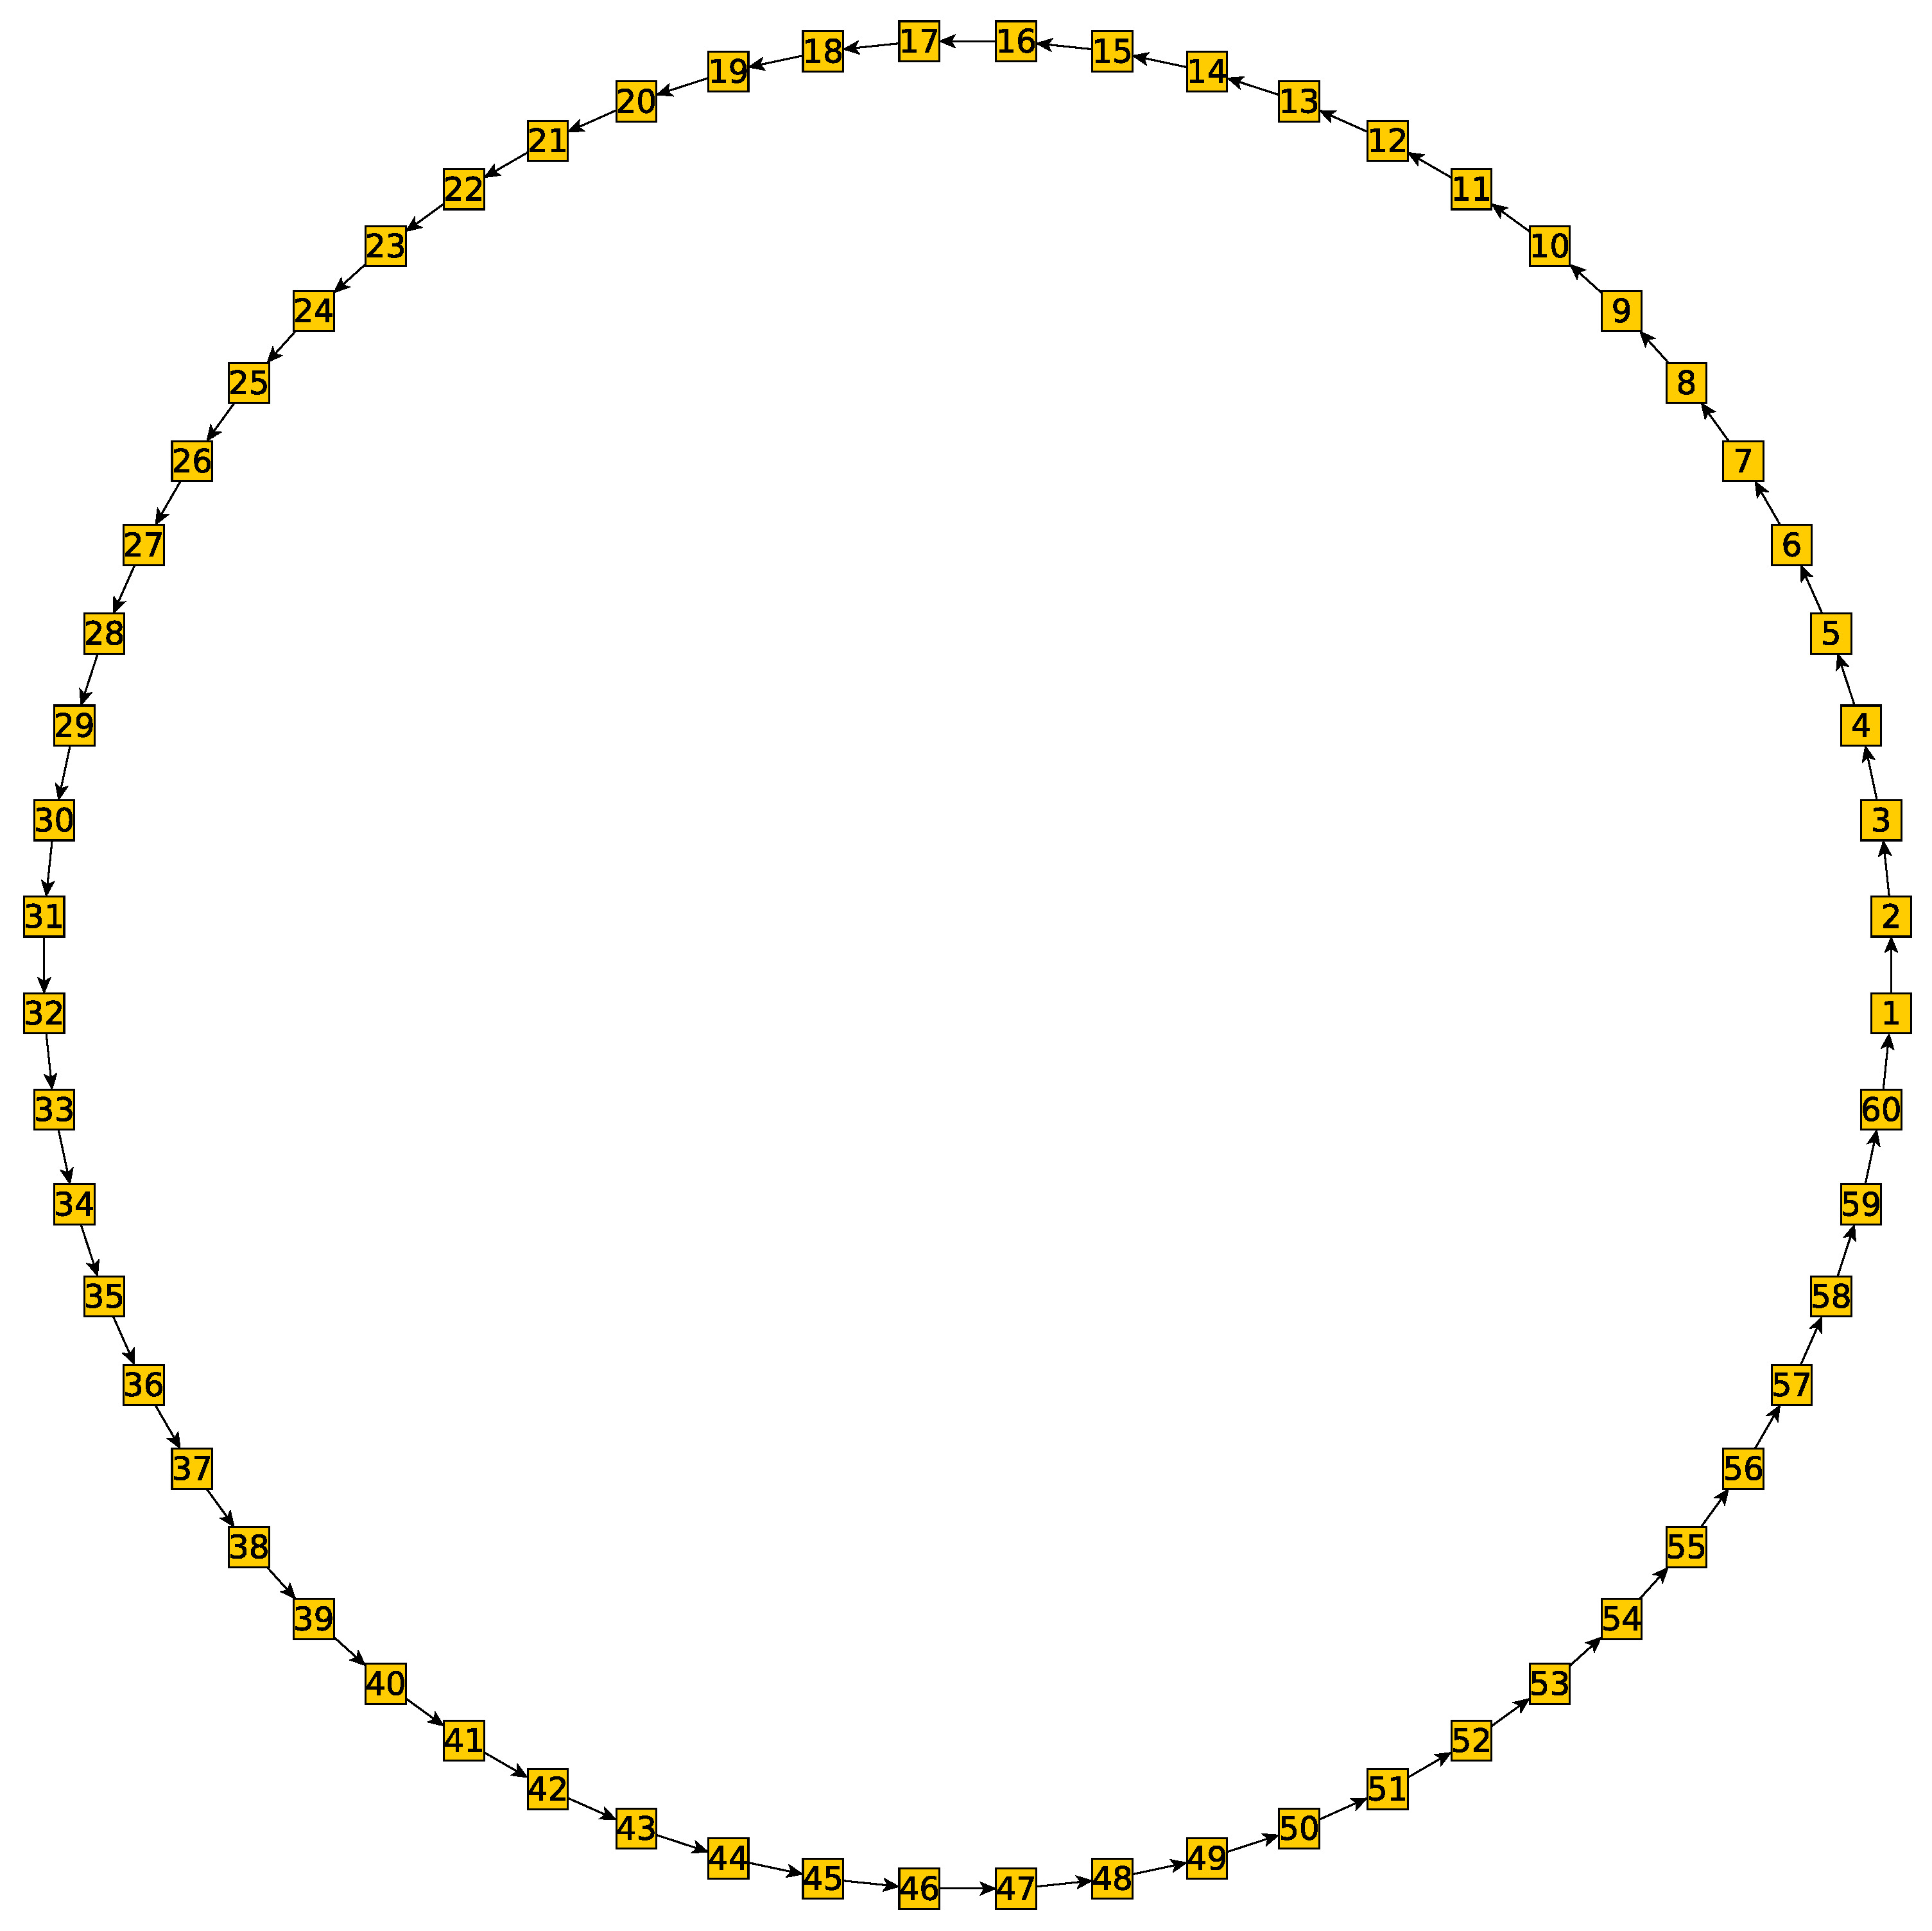
\includegraphics[width=\textwidth]{figures/CircleTests/CircleTestIllustrations/Circle_Test_Graph-No_arc_labels_or_costs.pdf}}
	\caption{Circle Test Graph example with no arc labels or costs drawn in}
	\label{fig:ctgnaloc}
\end{figure}

\begin{figure}[thbp]
	\noindent
	\fbox{
		\parbox{\textwidth}{
			A1, A2, A3, A4, A5, A6, A7, A8, A9, A10, A11, A12, A13, A14, A15, A16, A17, A18, A19, A20, A21, A22, A23, A24, A25, A26, A27, A28, A29, A30, A31, A32, A33, A34, A35, A36, A37, A38, A39, A40, A41, A42, A43, A44, A45, A46, A47, A48, A49, A50, A51, A52, A53, A54, A55, A56, A57, A58, A59, A60
		}
	}
	\caption{Best possible genome for the supplied Circle Test example}
	\label{fig:bpgftscte}
\end{figure}

While using the circle test data set might not give an exact answer to what configuration of the parameters is optimal, it still gives a usable prediction of what configurations work in a general case with the implementation. Another limitation that is not addressed at this point is that it only makes sense to evaluate it as giant round trip completed by one vehicle. It could be adopted to facilitate testing splitting the graph between several vehicles by adding a depot node in the center and making edges that are not required to service from it to all the nodes (as illustrated in figure \ref{fig:ctgcdnaoeloc}). However that would add a lot of complexity, and it would not be feasible to investigate it further at this point.

\begin{figure}[thbp]
	\centerline{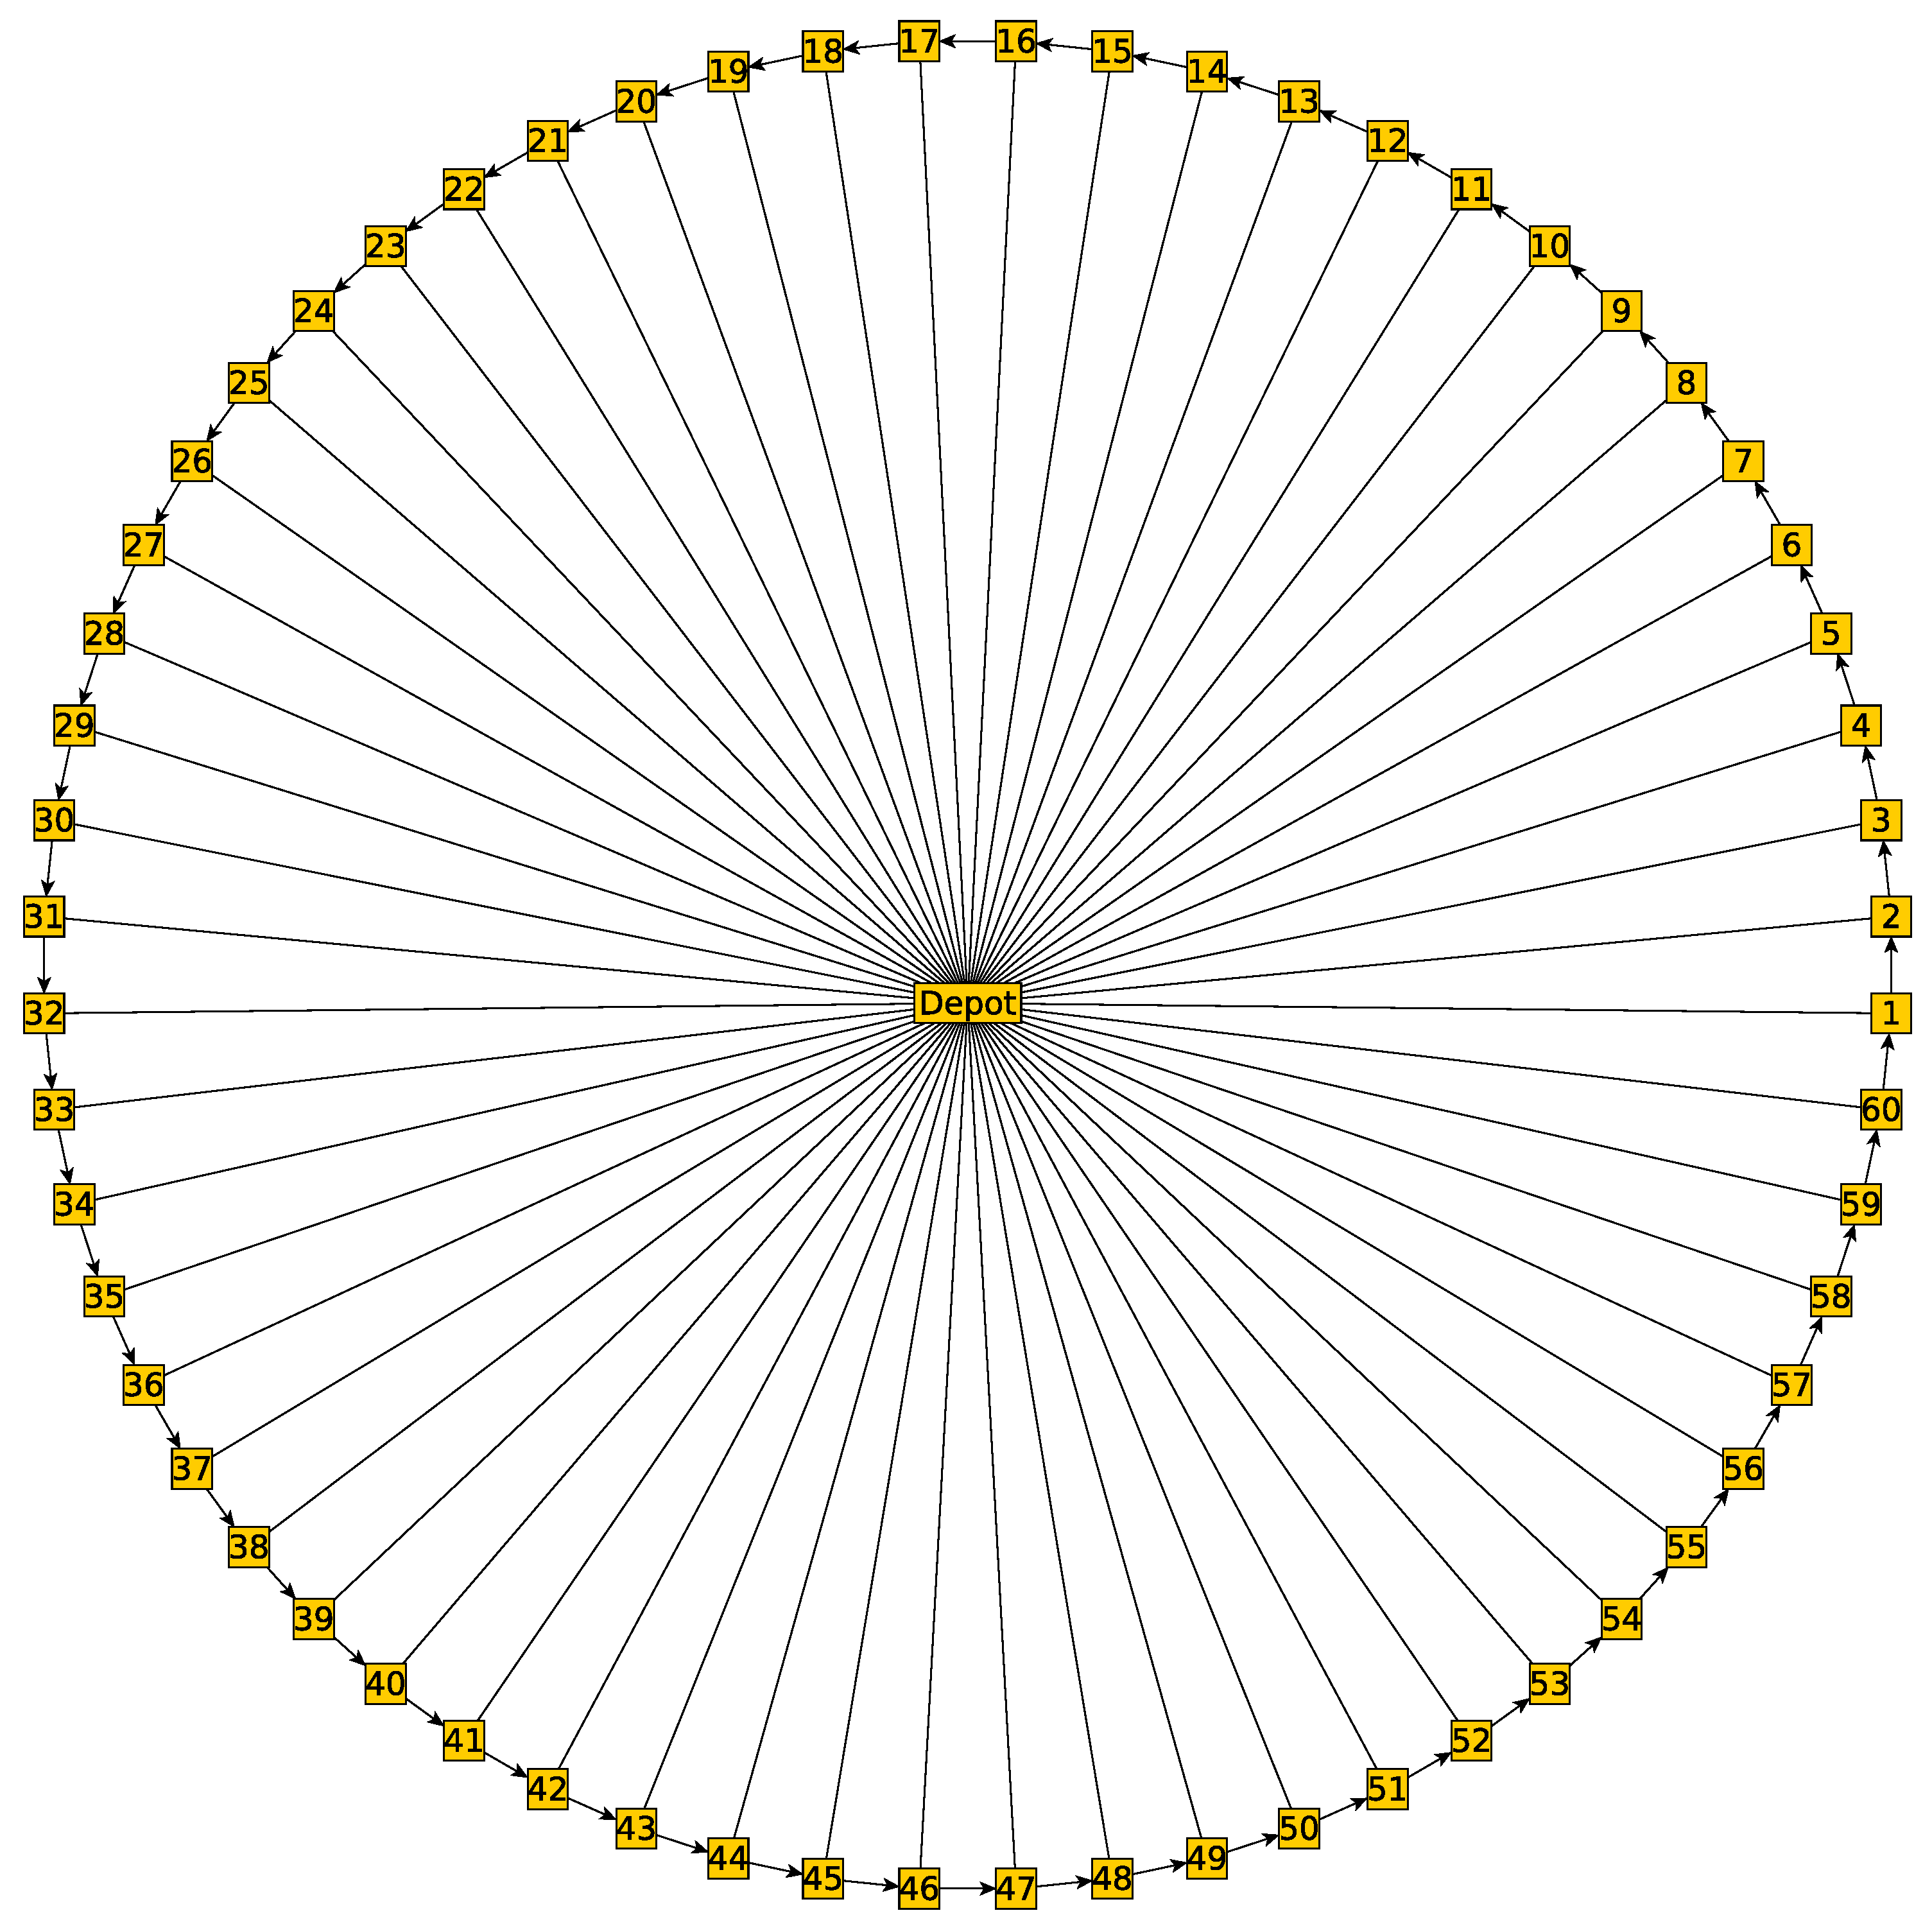
\includegraphics[width=\textwidth]{figures/CircleTests/CircleTestIllustrations/Circle_Test_Graph_Central_Depot-No_arc_or_edge_labels_or_costs.pdf}}
	\caption{Alternative Circle Test Graph example with depot node and no arc labels or costs drawn in}
	\label{fig:ctgcdnaoeloc}
\end{figure}

%Comment on memeticism here?

% section experimental_plan (end)

\section{Experimental Setup} % (fold)
\label{sec:experimental_setup}
% This section should be about how we did the experiments, ie. what parameters we used and so forth
The tuning of the MA was split into three parts. Determining the population size, parent selection, and adult selection. 
For each part, a set of parameters to be tested were selected based on the author's previous experience with tuning EAs and the size of the problem at hand. Then each configuration was to be ran 30 times to gather data about the best results found under the configuration, and the population averages. To make the results as comparable as possible, it was chosen to let each configuration run for exactly 100000 generations. For each run all the genotypes were initialized randomly, and each 16th generation the best fitness of the population, the average fitness of the population, and the standard deviation of the fitness of the population at that point was recorded.

For determining the population size, it was decided to try population sizes corresponding to 10\%, 50\%, 100\%, and 200\% of the genome length. When testing it uniform selection was used for parent selection, and full generational replacement for the adult selection.

When testing the parent selection the size of the population was set at 200\% of the genome length, and full generational replacement was used for the adult selection, as that allowed us to reuse the results from the population size run for uniform selection.

When trying to find the best way to do the adult selection a population size of 200\% of the genome length, and fitness proportionate selection as the parent selection were used. When testing overproduction it was decided to make as many pairs as there are individuals in the population, ie. producing twice as many children as there can be survivors to next generation.

During the determination of whether random mutation or using hill climbing for mutation it was decided to use a population size of 200\% of the genome length, fitness proportionate adult selection, and overproduction as the adult selection.

% section experimental_setup (end)

\clearpage

\section{Results} % (fold)
\label{sec:results}

Now that the experimental plan has been outlined, in this section the results will be presented. First the initial results for the population size experiment will be shown. Then the outcome of using different parameters for the parent selection is going to be laid out. After that the experimental results when testing different configurations for mutation are going to be presented. Finally, the results form a follow up experiment on the population size will be shown.

\subsection{Population Size} % (fold)
\label{sub:population_size}

When observing the results from the population size test runs, it can be noticed that that a lower population size yields better results. In figure \ref{fig:ctpab} it can be seen that the larger populations perform noticeably worse, with the largest population (120 individuals) getting a fitness value of around 700 by the end of the runs, while the smallest population size (6 individuals) end up with a fitness of about 600.

A possible reason for this is that uniform selection combined with full generational replacement is not biased in any way. This makes it very random in terms of that the fintess of the individuals in the existing population will not affect future generations. The population will however be influenced by the previous generations in terms of that their genomes will be combinations of previous genomes with mutations.

A possible explanation then could be in that the best individual from each generation is kept, and is injected in place of the worst one at the end of each generation. This will have a hughe impact in a tiny population of only 6 individuals, effectively dragging the population towards the currently best. But as population sizes increase the best individual and its offspring have less impact on the average of the population.

This effect should be offset by introducing bias in the population towards that the individuals with better fitness have a better chance at impacting future generations. But just to be certain that this is a quirk of combining uniform selection, full generational mixing, and the constant reintroduction of the previous best single individual at the cost of the currently worst, a control experiment for parent size using another form of parent selection and generational replacement was set up.

\begin{landscape}
\begin{figure}[thbp]
	\centerline{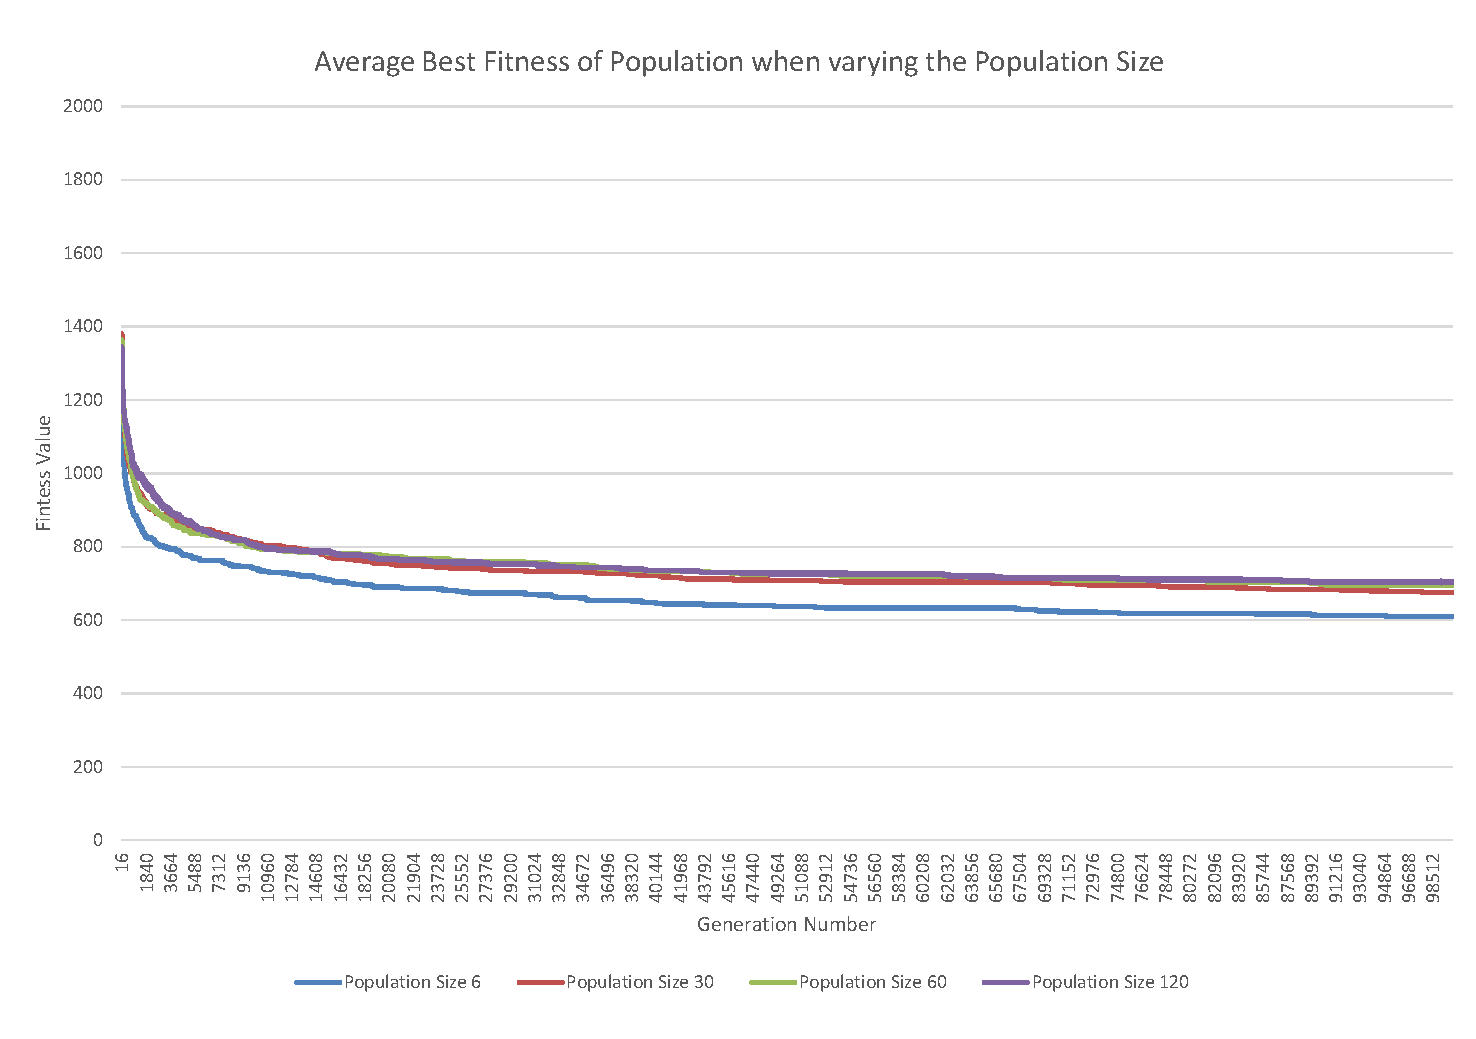
\includegraphics[height=0.945\textwidth]{figures/CircleTests/PopulationSize/CircleTestsPopulationAverageBest.pdf}}
	\caption{Population Size - Average Best}
	\label{fig:ctpab}
\end{figure}
\end{landscape}

\begin{landscape}
\begin{figure}[thbp]
	\centerline{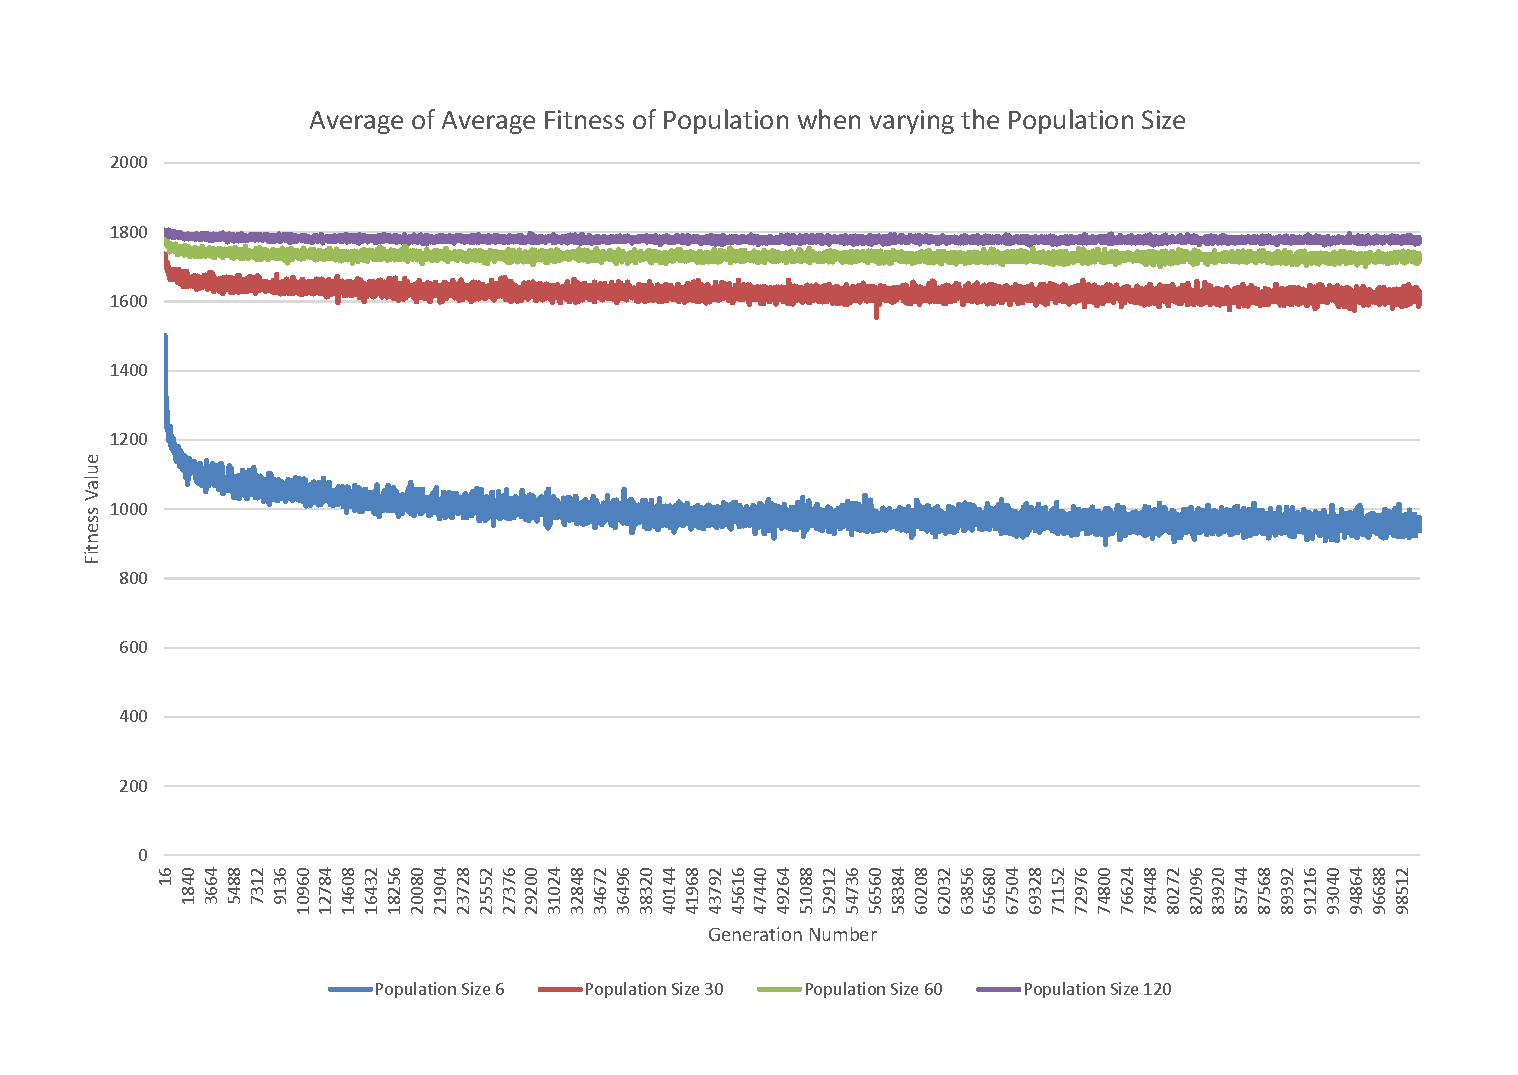
\includegraphics[height=0.945\textwidth]{figures/CircleTests/PopulationSize/CircleTestsPopulationAverageAverage.pdf}}
	\caption{Population Size - Average Average}
\end{figure}
\end{landscape}

\begin{landscape}
\begin{figure}[thbp]
	\centerline{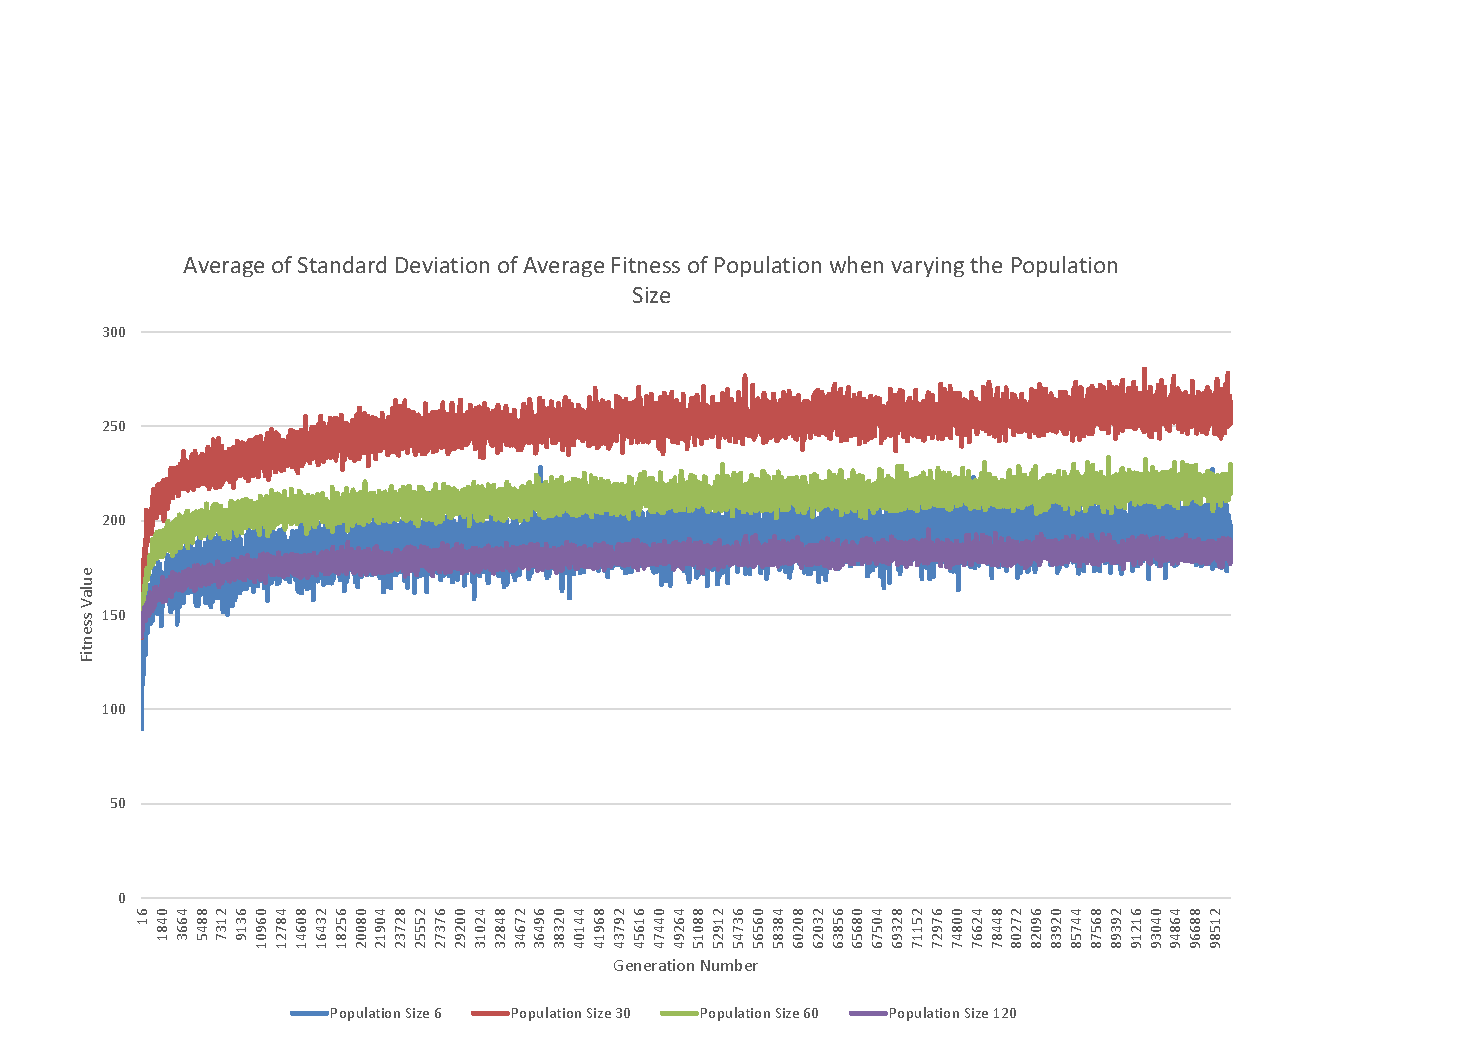
\includegraphics[height=0.945\textwidth]{figures/CircleTests/PopulationSize/CircleTestsPopulationAverageStandardDeviation.pdf}}
	\caption{Population Size - Average Standard Deviation}
\end{figure}
\end{landscape}
% subsection Population Size (end)

\clearpage

\subsection{Parent Selection} % (fold)
\label{sub:parent_selection}

In figure \ref{fig:ctpsab} it can be seen that fitness proportionate selection with a final fitness of just below 500 is clearly better than the tournament selection that reaches a fitness a bit above 500, which in turn finds better results on average than uniform selection with a fintess of about 700. The averages fitness of each populations average seem to quickly decrease before beginning to decrease slowly for tournament and fitness proportionate selection, while the uniform selection shows only a very slow improvement over time.

\begin{landscape}
\begin{figure}[thbp]
	\centerline{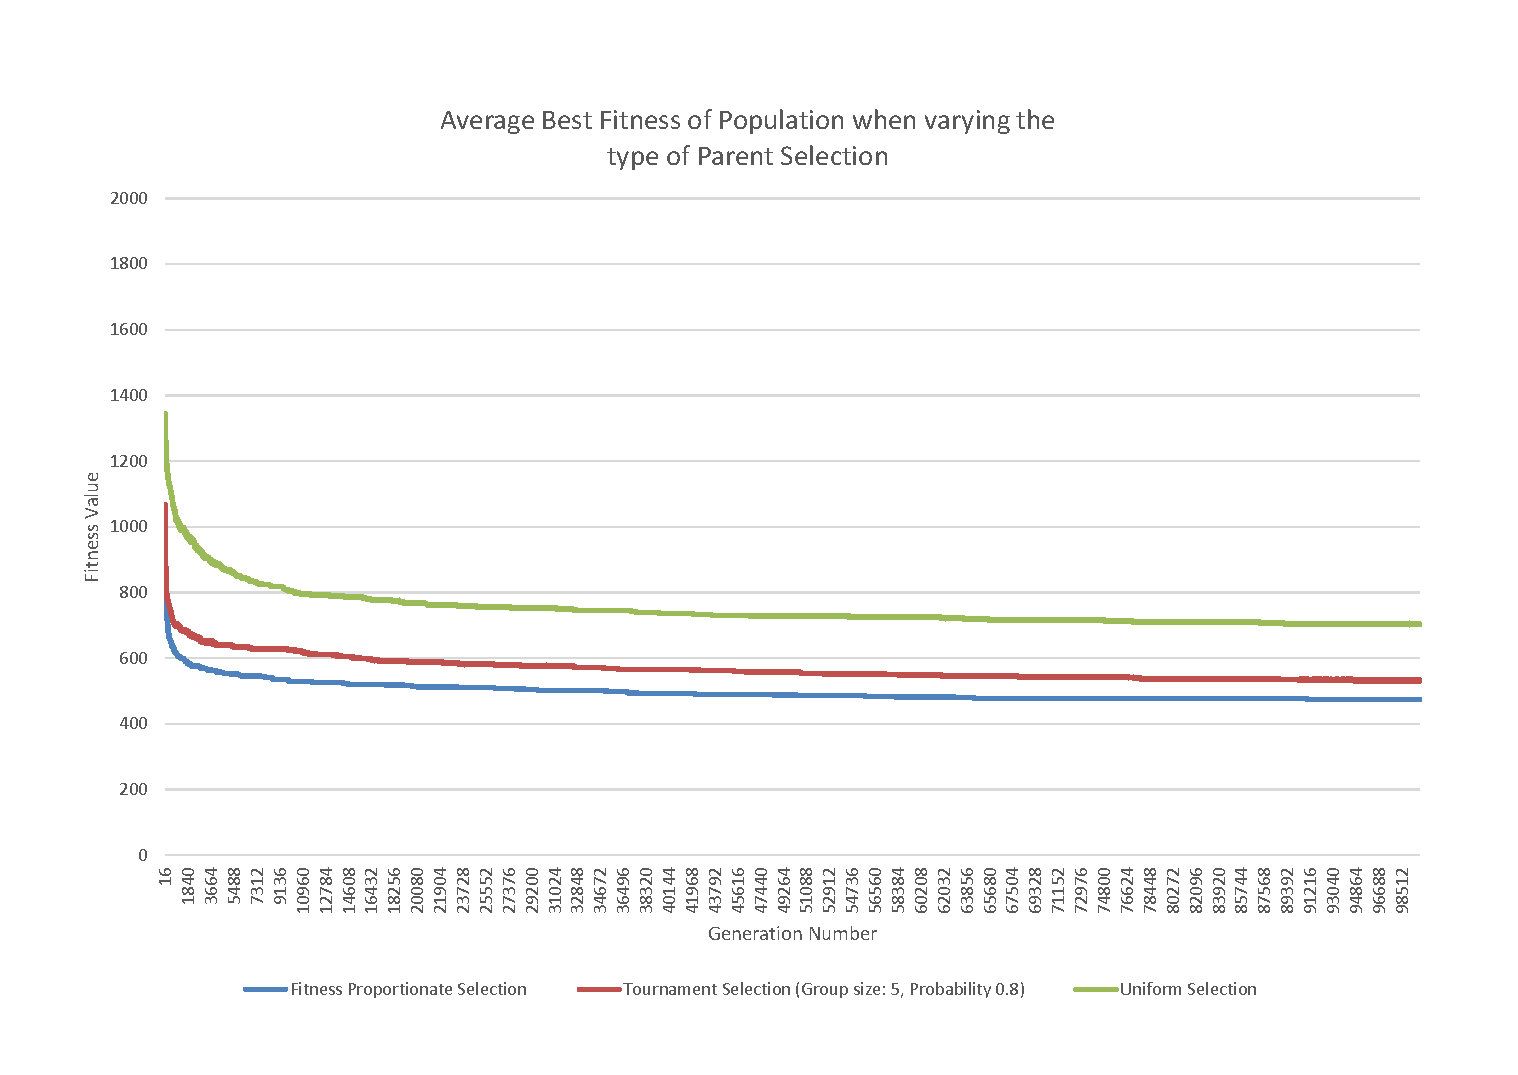
\includegraphics[height=0.945\textwidth]{figures/CircleTests/ParentSelection/CircleTestParentSelectionAverageBest.pdf}}
	\caption{Parent Selection - Average Best}
	\label{fig:ctpsab}
\end{figure}
\end{landscape}

\begin{landscape}
\begin{figure}[thbp]
	\centerline{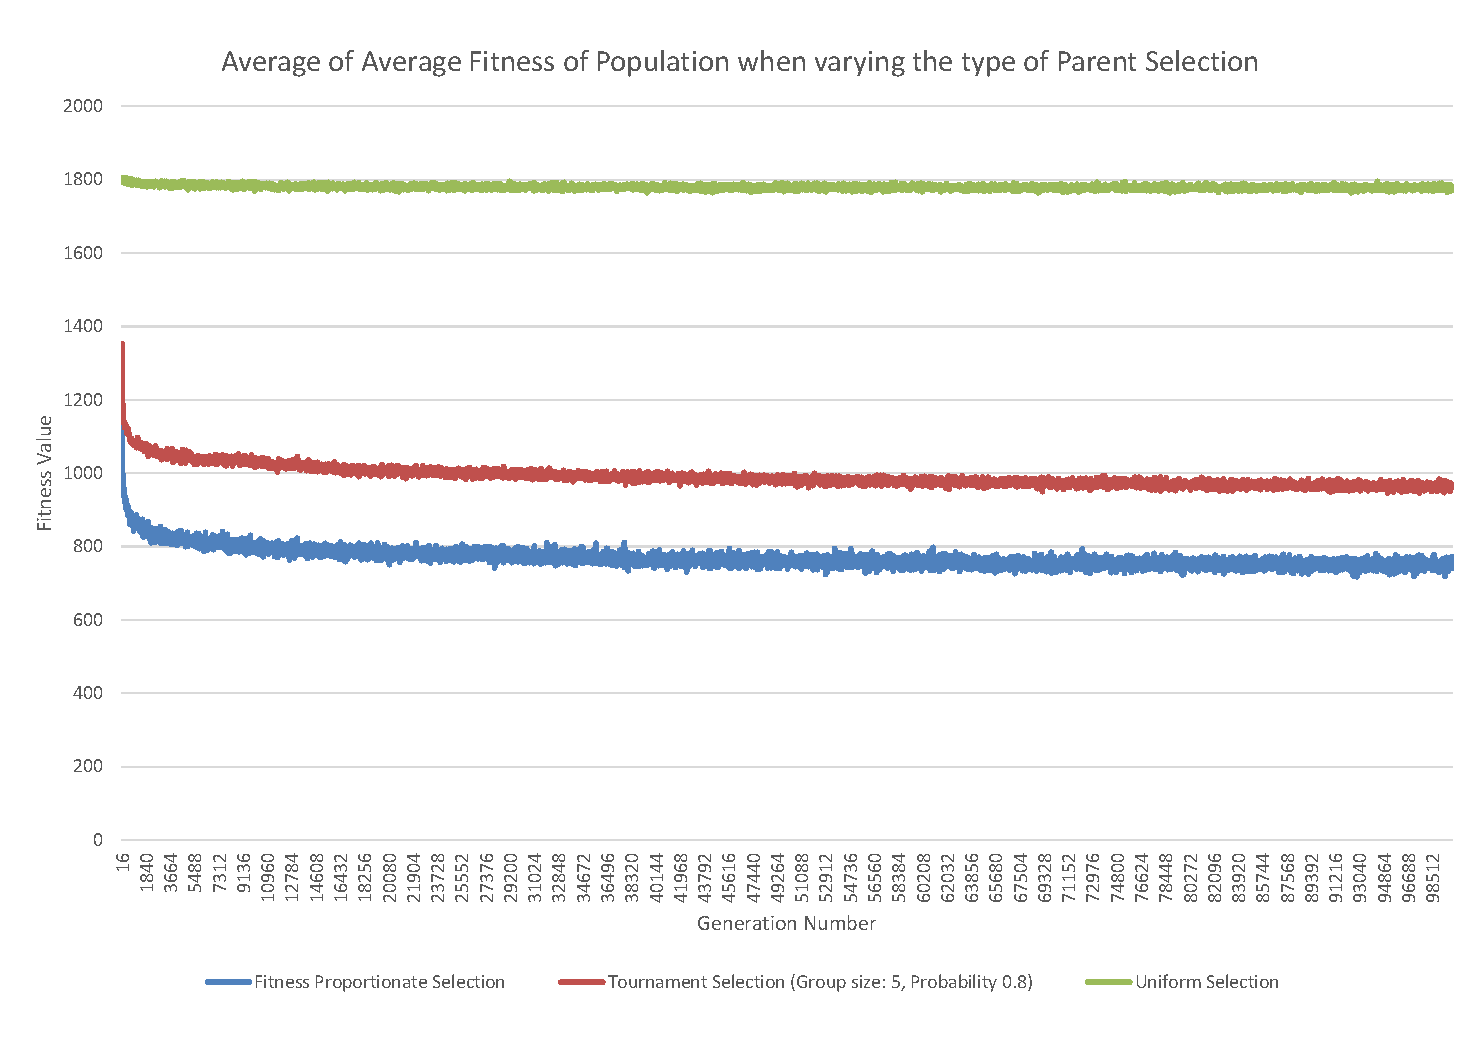
\includegraphics[height=0.945\textwidth]{figures/CircleTests/ParentSelection/CircleTestParentSelectionAverageAverage.pdf}}
	\caption{Parent Selection - Average Average}
\end{figure}
\end{landscape}

\begin{landscape}
\begin{figure}[thbp]
	\centerline{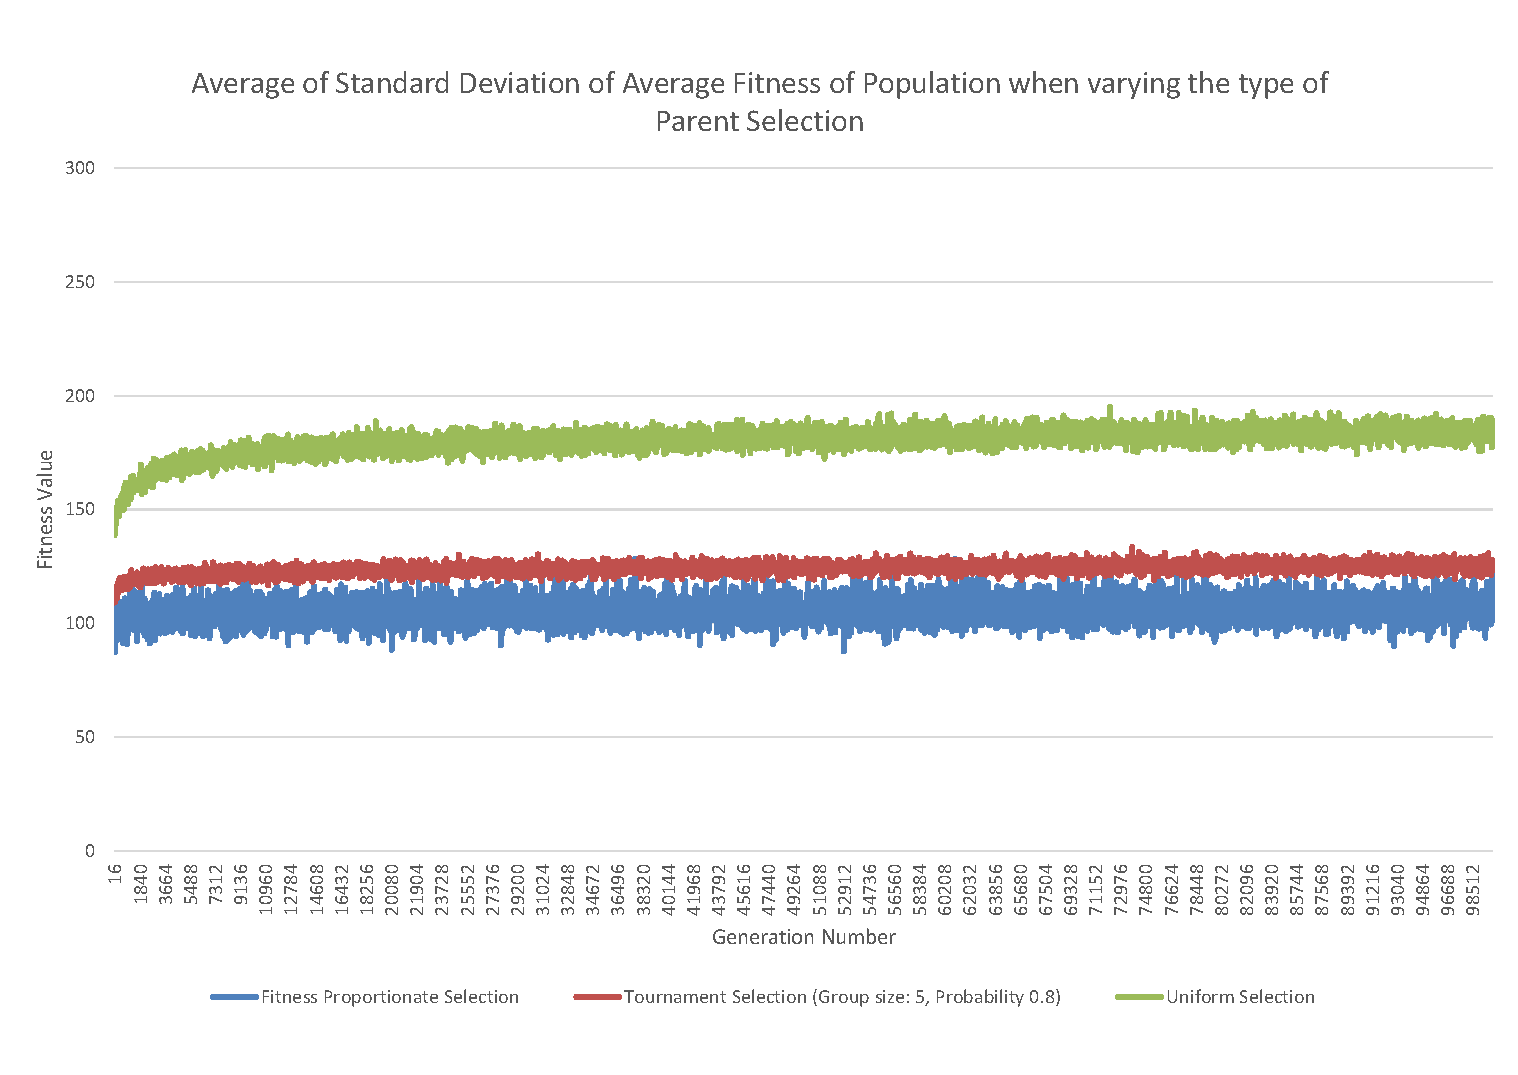
\includegraphics[height=0.945\textwidth]{figures/CircleTests/ParentSelection/CircleTestParentSelectionAverageStandardDeviation.pdf}}
	\caption{Parent Selection - Average Standard Deviation}
\end{figure}
\end{landscape}
% subsection parent_selection (end)

\clearpage

\subsection{Adult Selection} % (fold)
\label{sub:adult_selection}

When looking at the results for the adult selection in figure \ref{fig:ctasab}, the most striking thing is that completely flat curve for the elitist mixing average best, indicating that there on average is no improvement at all in the best solutions found when using it as adult selection. This can be explained by observing that the average standard deviation in each population is 0 (figure \ref{fig:ctasasd}), coupled with that the average of fintess of the population being stuck on a single value in figure \ref{fig:ctasaa} indicating that all the individuals in the population have the same fitness. What has likely happened is that the population has become stuck in a local optimum, and all the individuals it produces are exact copies of the currently best found solution.

When looking for what adult selection gives the best output according to these results both overproduction and random mixing give better results than elitist mixing, and overproduction yields slightly better results than random mixing.

\begin{landscape}
\begin{figure}[thbp]
	\centerline{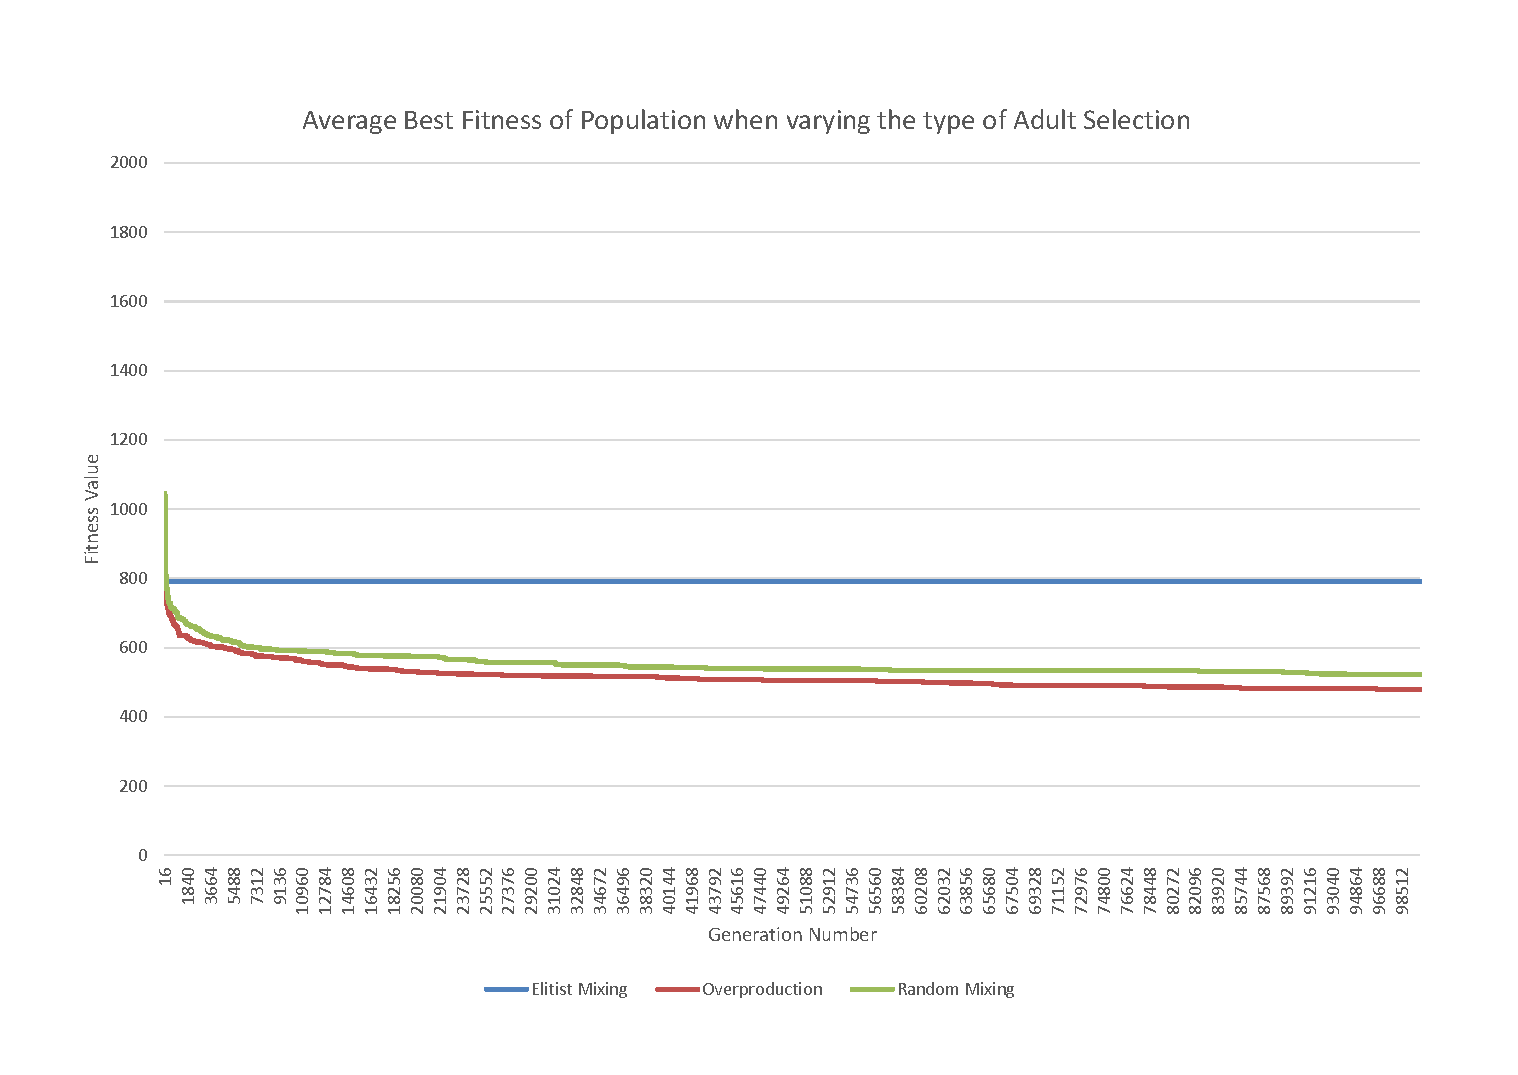
\includegraphics[height=0.945\textwidth]{figures/CircleTests/AdultSelection/CircleTestAdultSelectionAverageBest.pdf}}
	\caption{Adult Selection - Average Best}
	\label{fig:ctasab}
\end{figure}
\end{landscape}

\begin{landscape}
\begin{figure}[thbp]
	\centerline{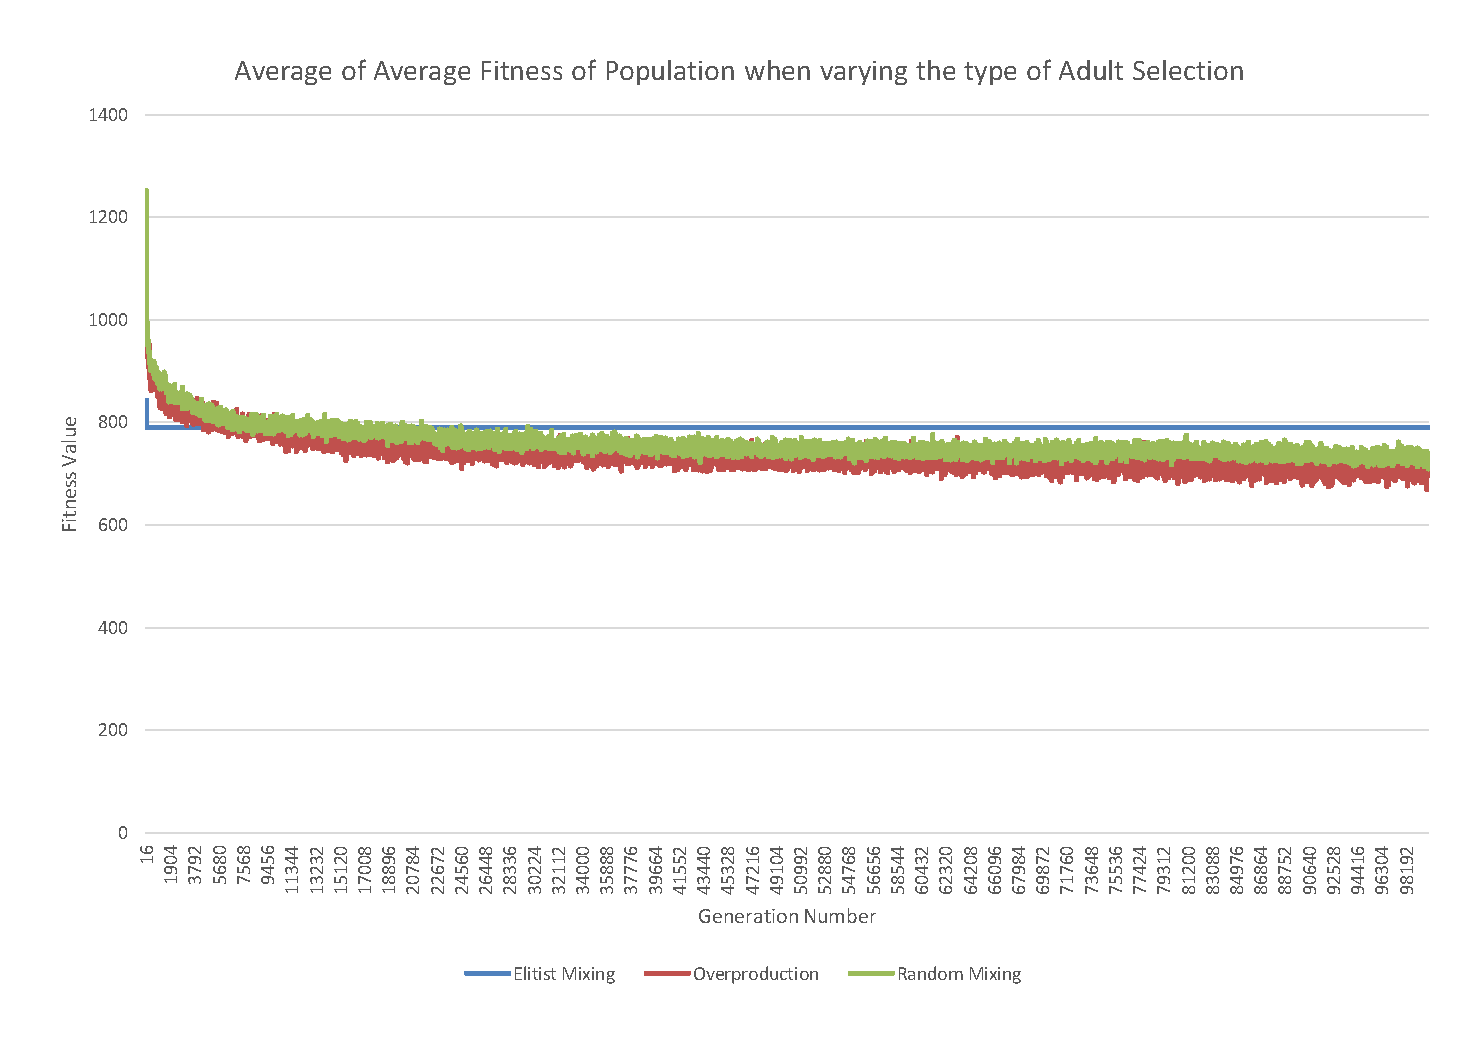
\includegraphics[height=0.945\textwidth]{figures/CircleTests/AdultSelection/CircleTestAdultSelectionAverageAverage.pdf}}
	\caption{Adult Selection - Average Average}
	\label{fig:ctasaa}
\end{figure}
\end{landscape}

\begin{landscape}
\begin{figure}[thbp]
	\centerline{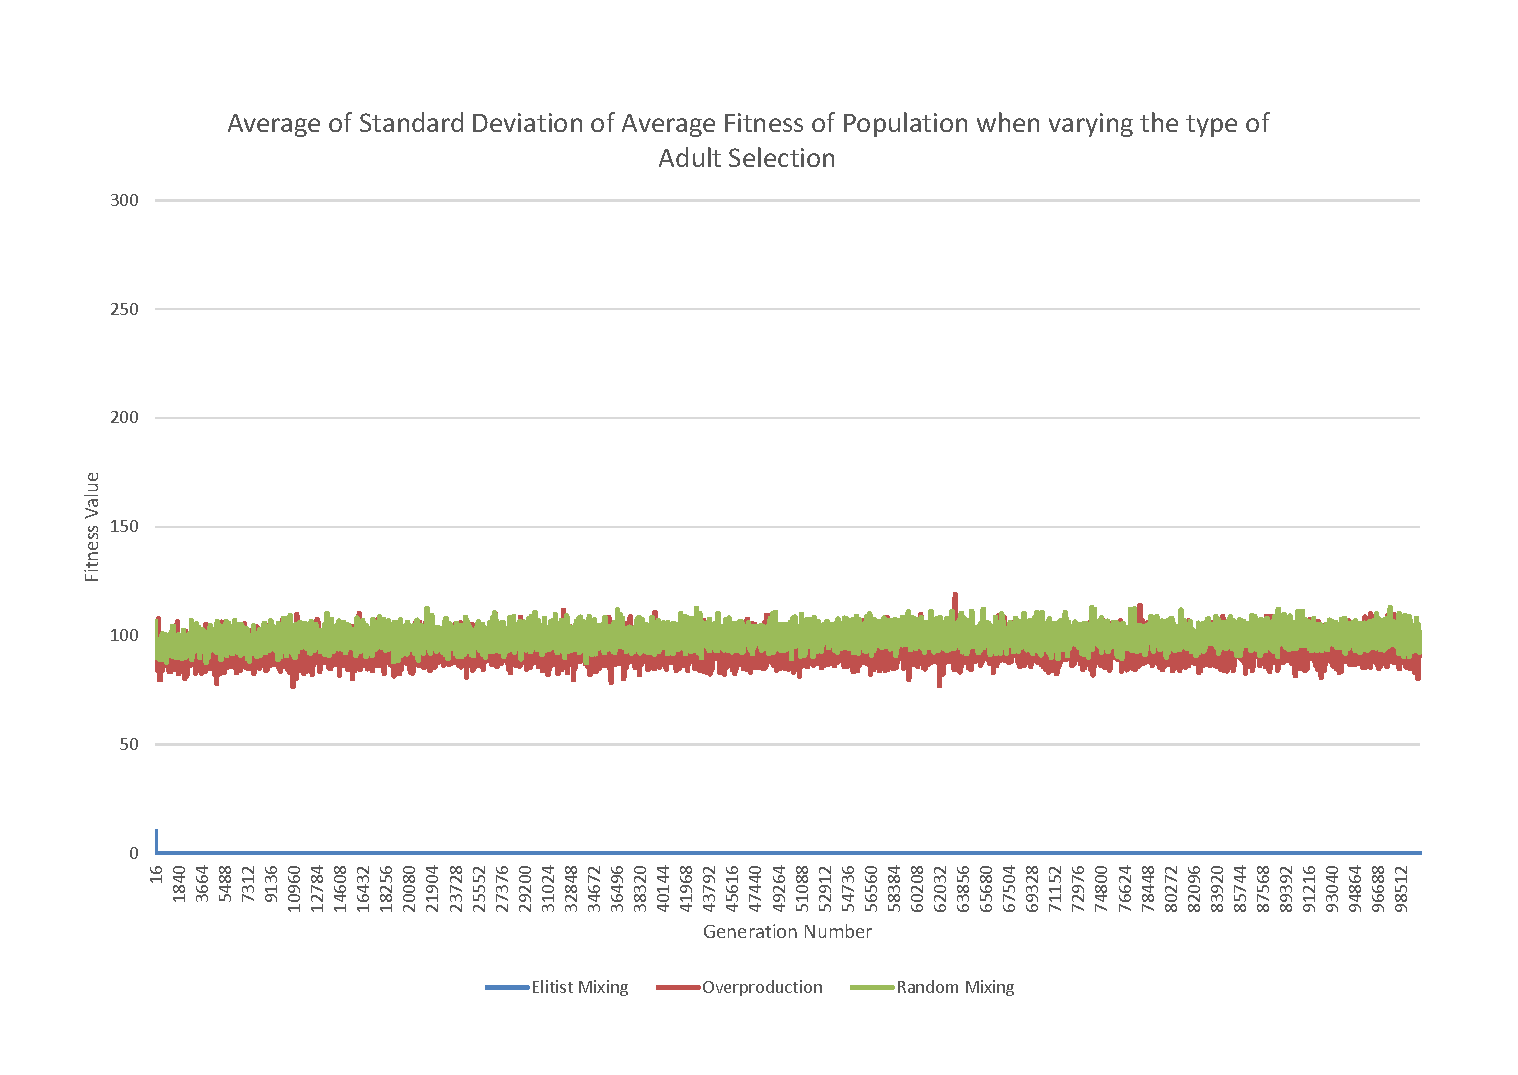
\includegraphics[height=0.945\textwidth]{figures/CircleTests/AdultSelection/CircleTestAdultSelectionAverageStandardDeviation.pdf}}
	\caption{Adult Selection - Average Standard Deviation}
	\label{fig:ctasasd}
\end{figure}
\end{landscape}
% subsection adult_selection (end)

\clearpage

\subsection{Mutation Types} % (fold)
\label{sub:mutation_types}

As can be seen from figure \ref{fig:ctmab} and \ref{fig:ctmaa} the memetic improvement yields better results than when doing random mutation. Adding a memetically improved child to the children before the adult selection seems to make little difference, though it reaches a tad better solutions a little bit earlyer than when not adding it. For both memetic approaches the fitness value tends to get as good as just below 400 in the long run, as can be seen in figure \ref{fig:ctmab}.

Figure \ref{fig:ctmasd} shows that the diversity of the population is somewhat lower when doing memetic improvement instead of random mutation.

\begin{landscape}
\begin{figure}[thbp]
	\centerline{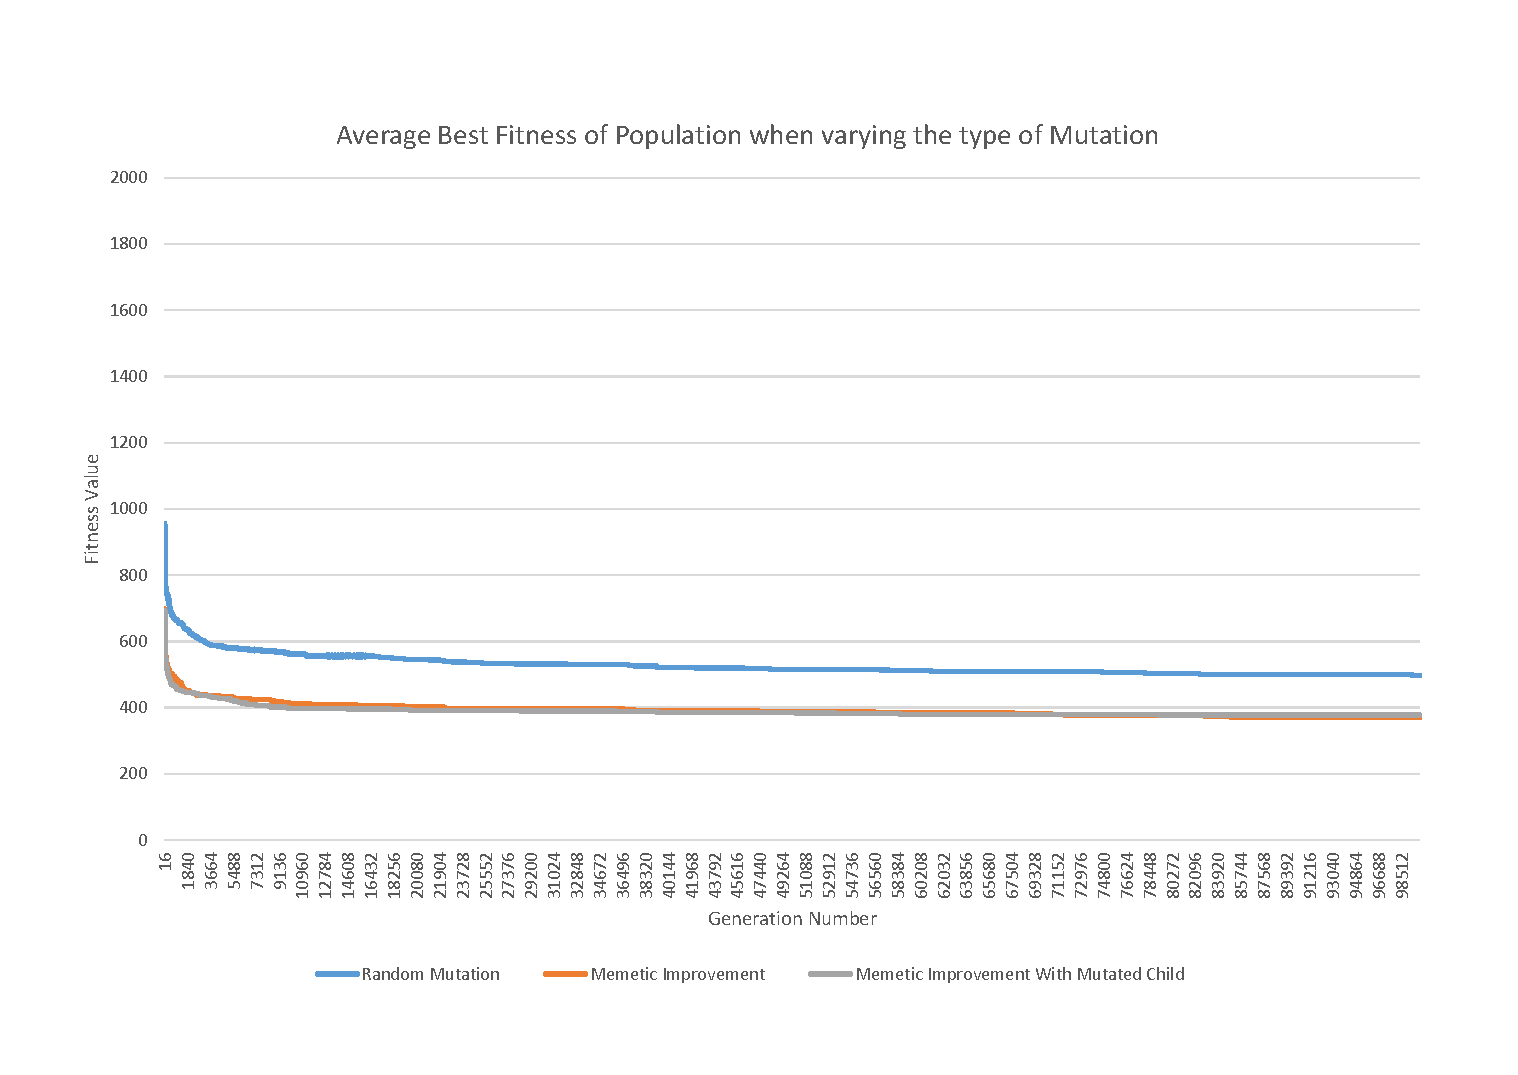
\includegraphics[height=0.945\textwidth]{figures/CircleTests/Mutation/CircleTestMutationAverageBest.pdf}}
	\caption{Mutation - Average Best}
	\label{fig:ctmab}
\end{figure}
\end{landscape}

\begin{landscape}
\begin{figure}[thbp]
	\centerline{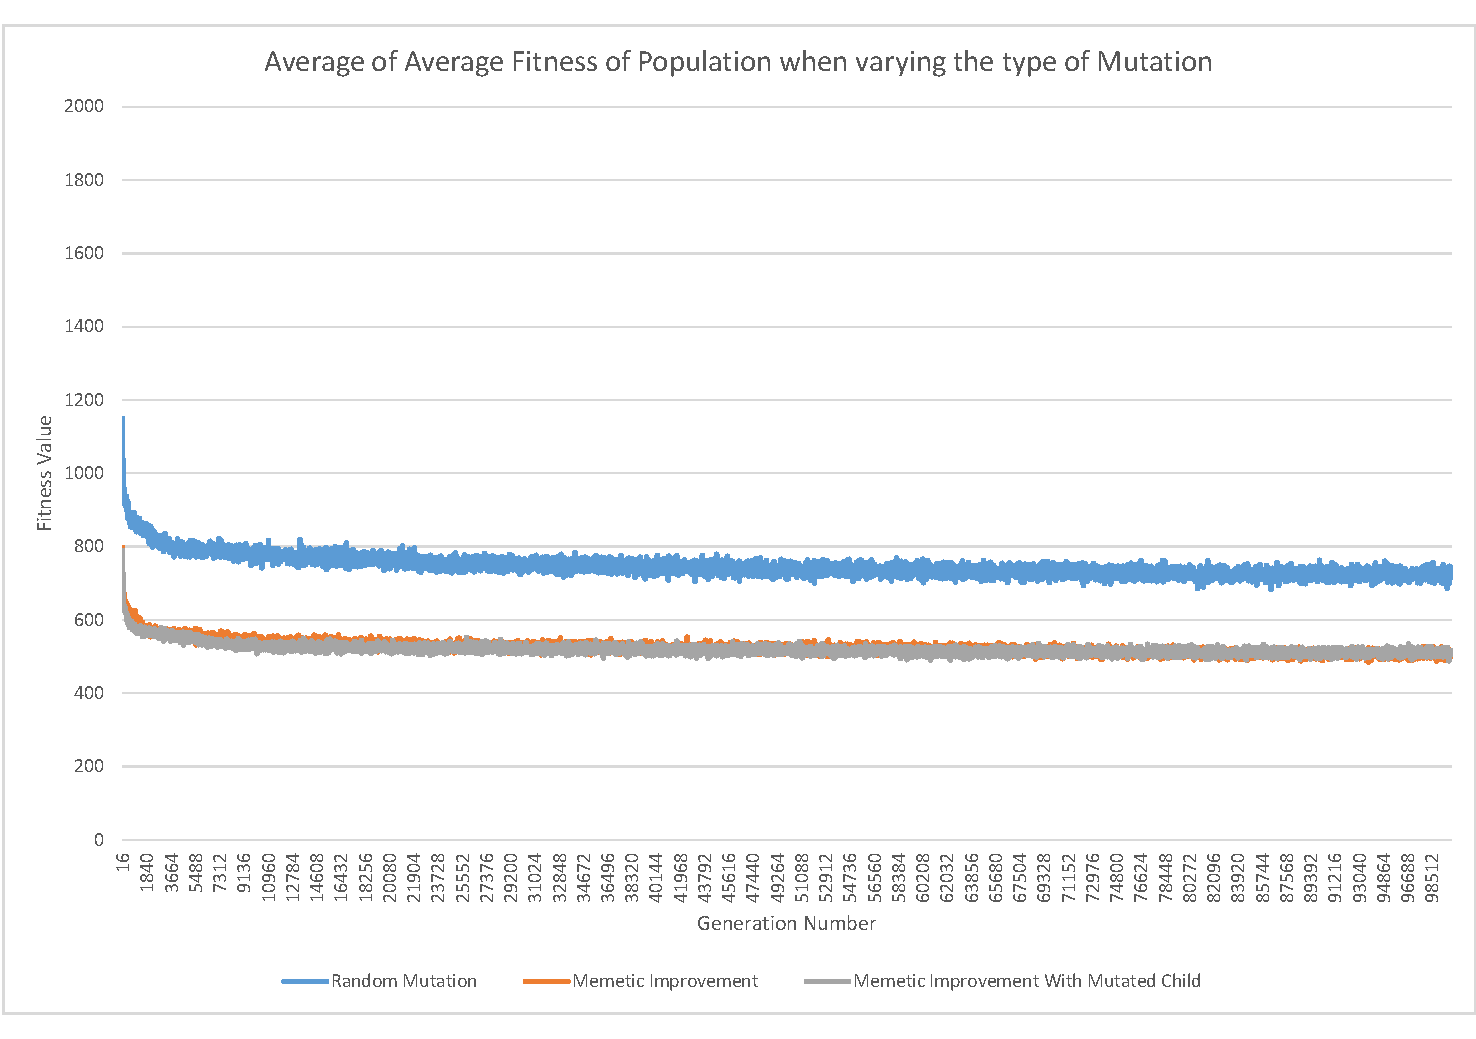
\includegraphics[height=0.945\textwidth]{figures/CircleTests/Mutation/CircleTestMutationAverageAverage.pdf}}
	\caption{Mutation - Average Average}
	\label{fig:ctmaa}
\end{figure}
\end{landscape}

\begin{landscape}
\begin{figure}[thbp]
	\centerline{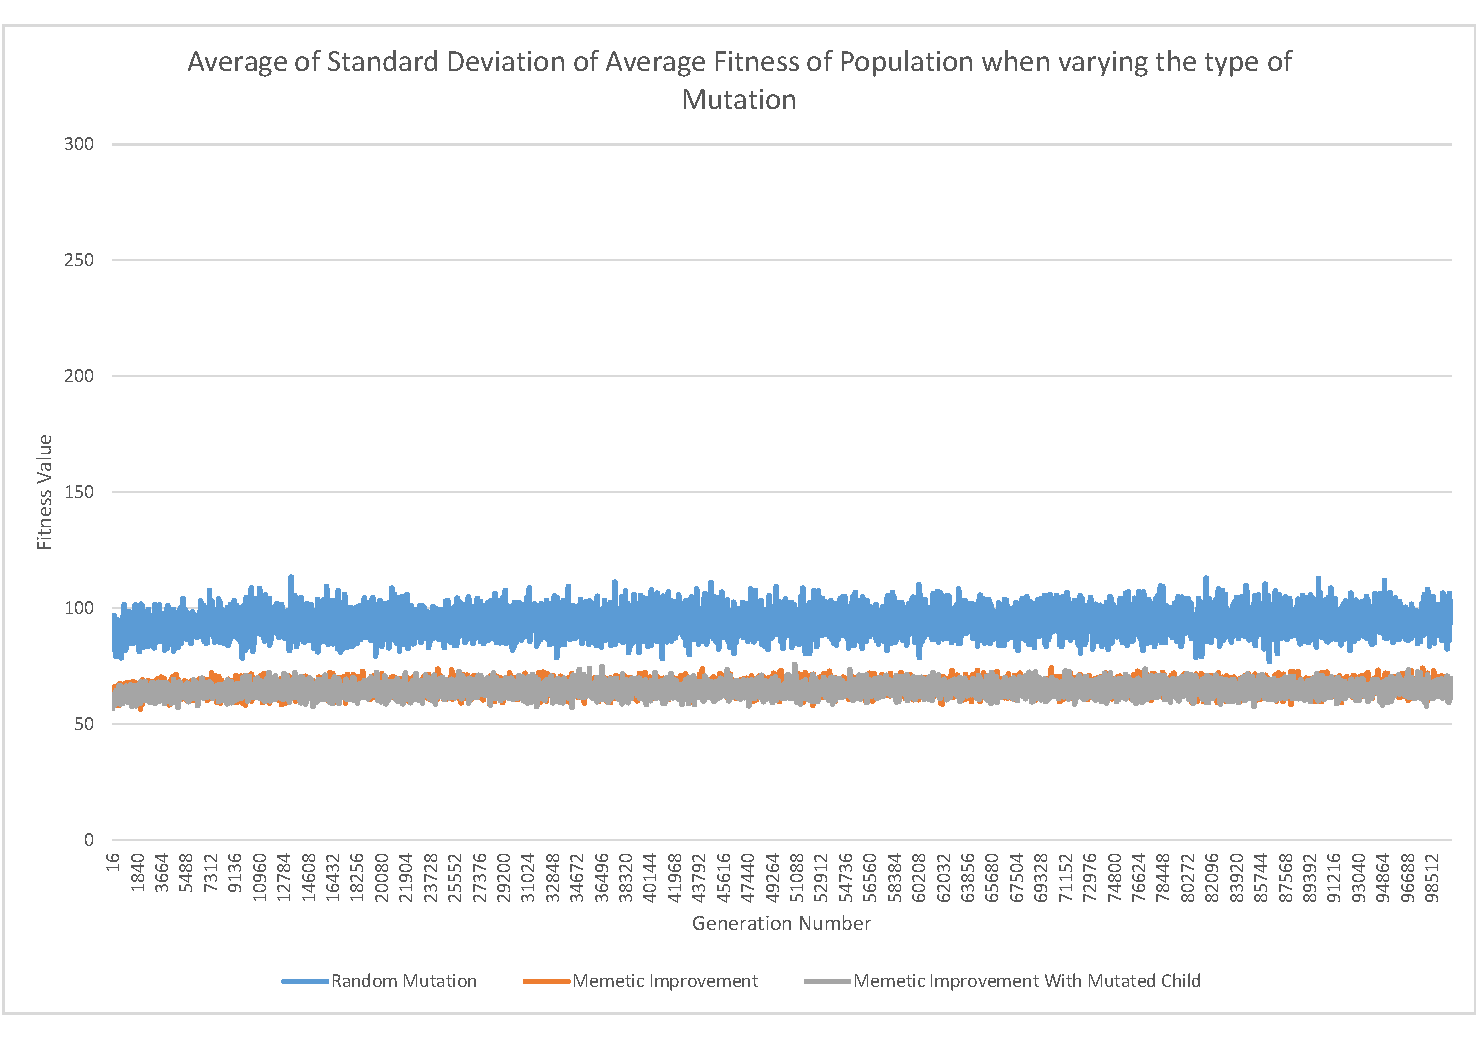
\includegraphics[height=0.945\textwidth]{figures/CircleTests/Mutation/CircleTestMutationAverageStandardDeviation.pdf}}
	\caption{Mutation - Average Standard Deviation}
	\label{fig:ctmasd}
\end{figure}
\end{landscape}
% subsection mutation_types (end)

\clearpage

\subsection{Population Size Control} % (fold)
\label{sub:population_size_control}

Due to the unexpected results in the population size tests (section \ref{sub:population_size}), it was decided to look into whether the effect of the population size could be impacted by the choice of uniform parent selection and full generational replacement. A control test was designed where each population was again run 30 times, but this time with fintess scaling selection and overproduction with twice as many children as the population size.

The results obtained here were according to the predictions about a bigger population size being generally better, and that the results when not guiding the direction of the population in any way are most likely due to the proportion of it that the best individual represents. A larger population gives better results, but as the populations grow very large there are diminishing returns on expanding it further. As can be seen in figure \ref{fig:cpscab} the largest population gives only marginally better results than the second largest population, which gives somewhat better results than the third largest population, which in turn gives a lot better results than the smallest population.

\begin{landscape}
\begin{figure}[thbp]
	\centerline{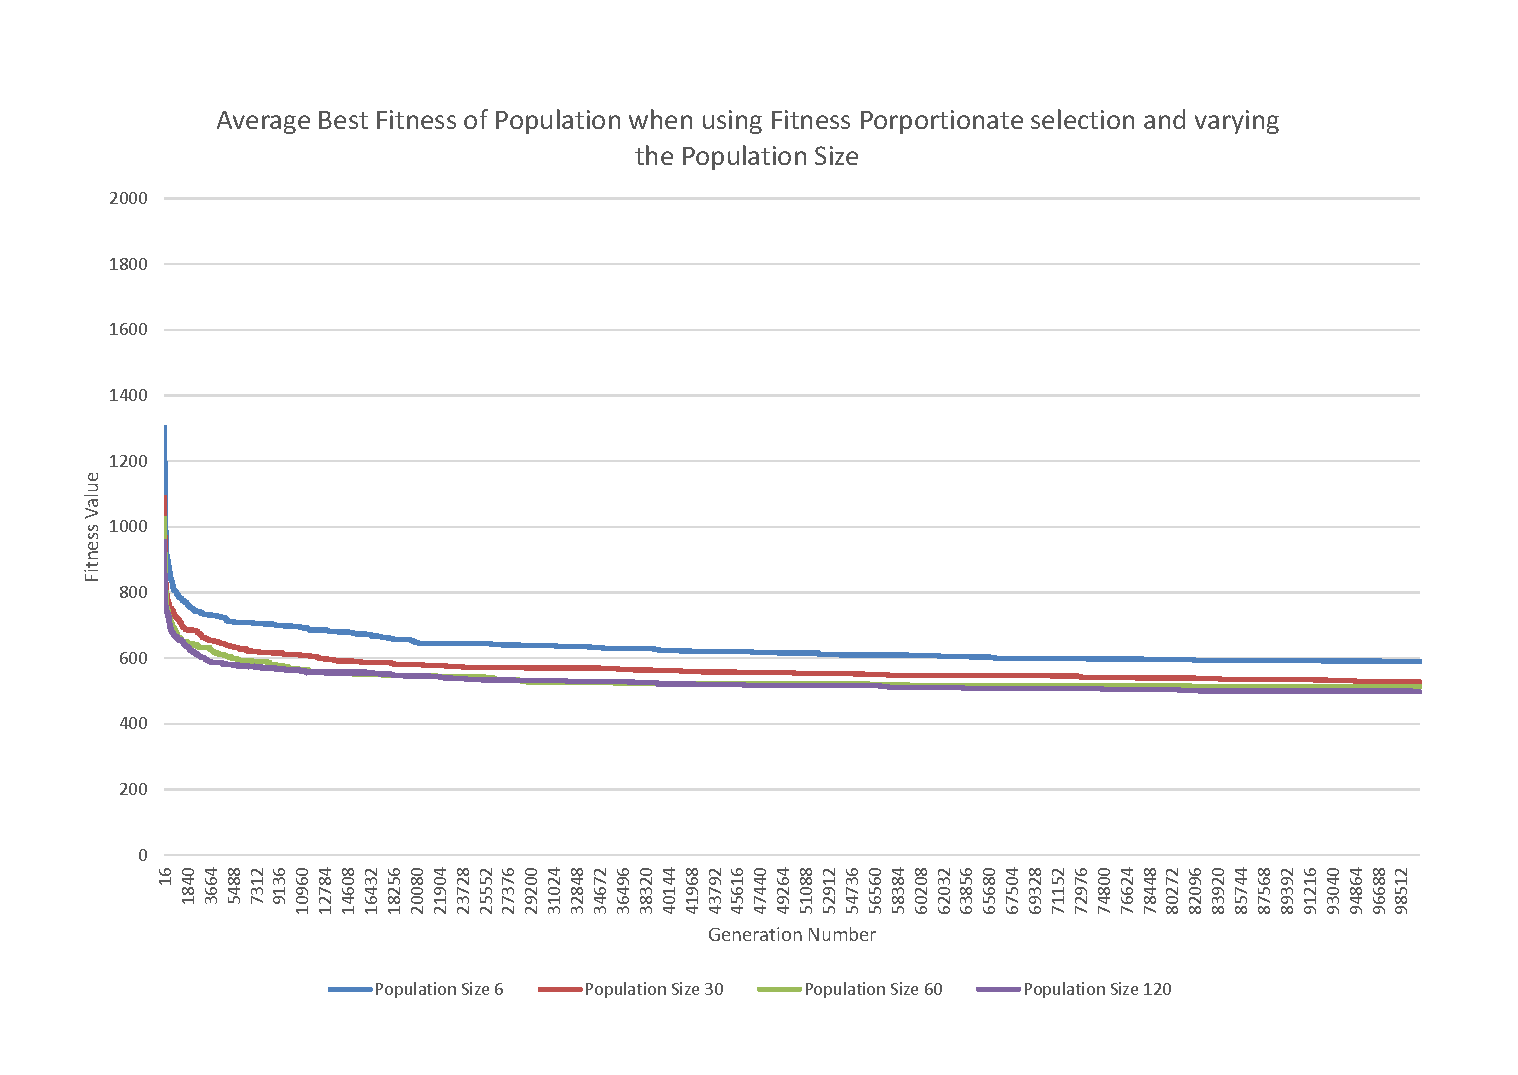
\includegraphics[height=0.945\textwidth]{figures/CircleTests/PopulationSizeControl/CirclePopulationSizeControllAverageBest.pdf}}
	\caption{Population Size Control - Average Best}
	\label{fig:cpscab}
\end{figure}
\end{landscape}

\begin{landscape}
\begin{figure}[thbp]
	\centerline{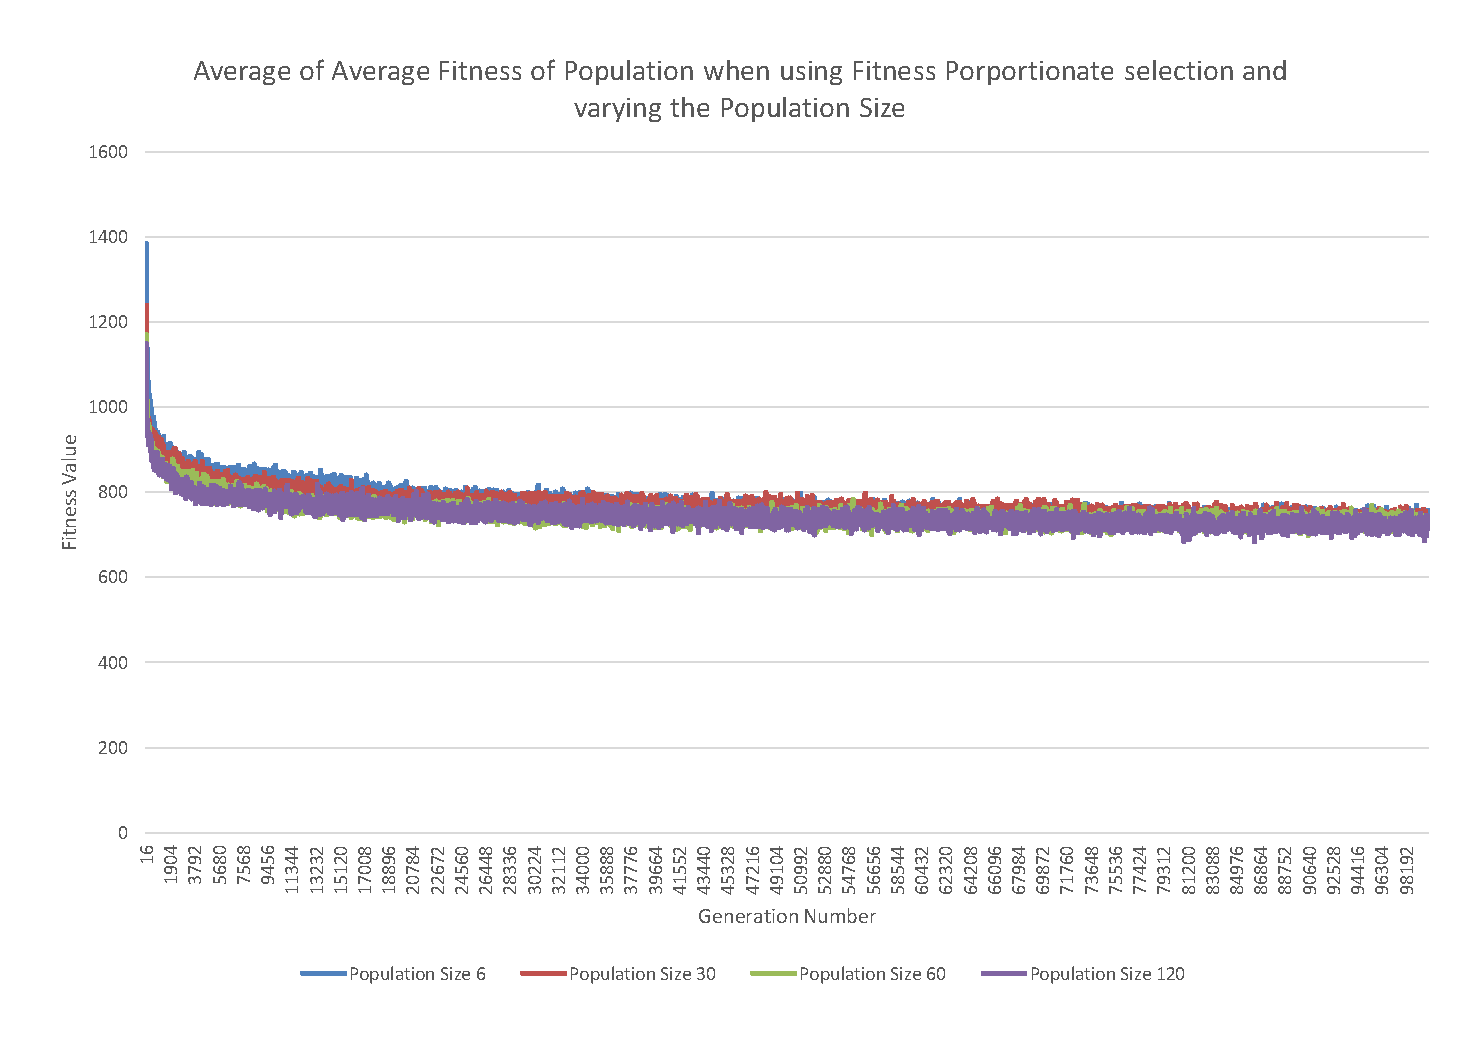
\includegraphics[height=0.945\textwidth]{figures/CircleTests/PopulationSizeControl/CirclePopulationSizeControllAverageAverage.pdf}}
	\caption{Population Size Control - Average Average}
\end{figure}
\end{landscape}

\begin{landscape}
\begin{figure}[thbp]
	\centerline{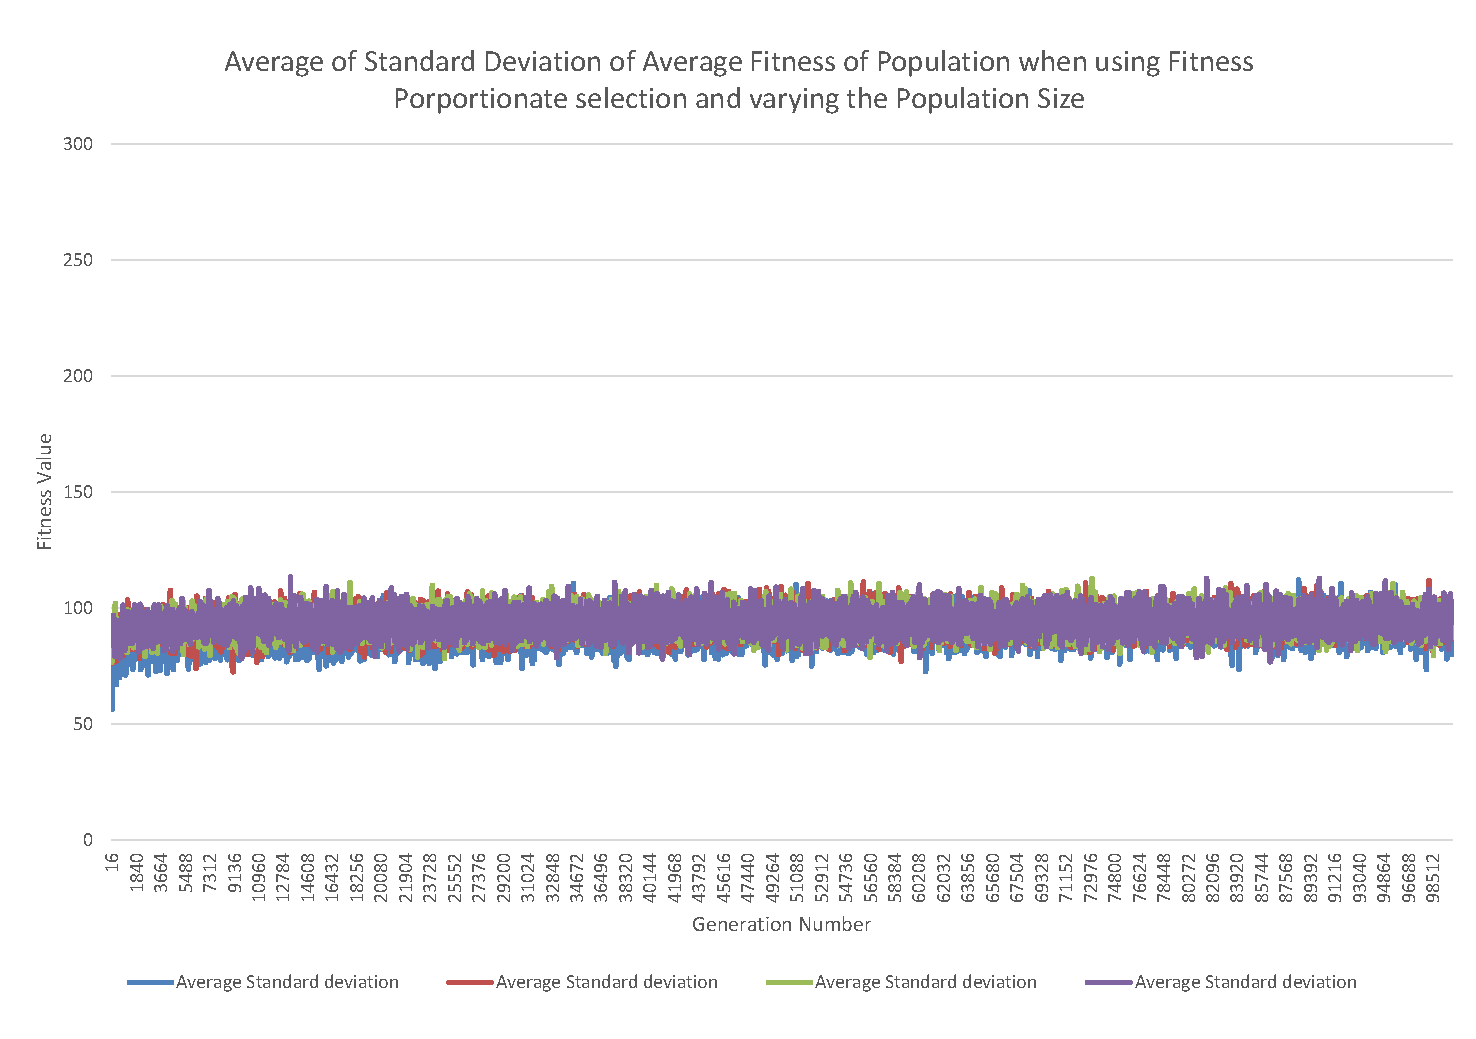
\includegraphics[height=0.945\textwidth]{figures/CircleTests/PopulationSizeControl/CirclePopulationSizeControllAverageStandardDeviation.pdf}}
	\caption{Population Size Control - Average Standard Deviation}
\end{figure}
\end{landscape}
% subsection population_size_control (end)

\clearpage

% section results (end)

\section{Evaluation and Conclusion} % (fold)
\label{sec:evaluation_and_conclusion}

The above experiments lead us to the following conclusions about the parameters for the MA. Section \ref{sub:parent_selection} indicated that the best parent selection method for the algorithm is fitness proportionate selection. As for the adult selection section \ref{sub:adult_selection} shows that overproduction is the adult selection type that gives the best fitnesses in the implementation. When it comes to the mutation tests in section \ref{sub:mutation_types}, it can be seen that memetic improvement gives much better results than random mutation.

In section \ref{sub:population_size_control} it is found that a larger population is better, but it has diminishing returns, and a population size of 200\% the length of the genome is not much better than a population size equivalent to 100\% the length of the genome. It contradicts the findings from section \ref{sub:population_size}, but it was found that those are most likely due to introducing the previous best each generation and the portion of the population it constitutes as populations grow smaller when no other form of elitism or directing of the population is present.

None of the configurations found an ideal solution with a fintess value of 60. The best fitness values the MA got were about 400 (found when doing the mutation configurations in section \ref{sub:mutation_types}) which is not too bad. The found fintess value indicates that the MA gives a solution that goes $\frac{400}{60} = 6.\overline{66} \approx 7$ times more than it needs around the circle. Considering that this can be achieved by switching the order of 7 pairs in the circle the quality of the solutions while not optimal are still acceptable.

Overall the experiments ran smoothly, usable results were obtained, and more importantly all of the results above are 100\% reproducible beacause all the configurations and random-seeds of each run of each experiment were kept.

What could be improved: A test that also tests splitting would be better. Using real world test data would give inidcations as to running time, which would make it better in itself. Furthermore it could give more parameters. Another signifficant limitation is that other configurations of the tournament selection were not looked into.

{
\rowcolors{2}{gray!15}{white}
\begin{table}[tbph]
\centering
\begin{tabular}{rl}
\toprule
\textbf{MA Parameter} & \textbf{Best found setting}     \\ \midrule
Parent selection      & Fitness proportionate selection \\
Adult selection       & Overproduction                  \\
Mutation type         & Memetic improvement             \\
Population size       & 200\%                           \\ \bottomrule
\end{tabular}
\caption{The tunable parameters in the MA and what settings were found to give the best results}
\label{tab:parameter_table}
\end{table}
}
% section evaluation_and_conclusion (end)
% chapter evolutionary_algorithm_configuration (end)

\cleardoublepage